\documentclass{article}
\usepackage[margin=2cm]{geometry}

\usepackage{cite}
\usepackage{graphicx}
\usepackage{wrapfig}
\usepackage{hyperref}
\usepackage{caption}
\usepackage{float}
\usepackage{setspace}
\usepackage{pdfpages}
\usepackage{adjustbox}
\usepackage{booktabs}
\usepackage{longtable}
\usepackage{pdflscape}

\title{Final Report}
\date{\today}

\begin{document}

\maketitle
\newpage
\tableofcontents   
\section{Overview of the Project}
% Approximate Word Count: 200 words

In this project I will try to develop a 4 dimensional variant of Tetris. The game will try to capture the essence of the original Tetris gameplay as well as the endless replayability while enhancing it with innovative new features. To find a balance in between the increased complexity provided by moving into higher dimensional spaces and the actual playability end enjoyability of the game, I will be limiting the 4 dimensional aspect to the Tetris pieces only. The player will see a 3 dimensional playing field that pieces fall into. Once they start rotating the 3 dimensional pieces they will notice that they are actually 3 dimensional slices of 4 dimensional collections of hypercubes. This will essentially just increase the number of possible rotations of the pieces and remove the rotational symmetry that is present in classic Tetris.
The goal is to create a fun fut complex game that lends itself to endless replayability as well as scientific exploration, just as Tetris did.

\section{Project Template Used}
% Approximate Word Count: 50 words
CM3030 Games Development Project Idea Title 1: Arcade Game

\section{Motivation}
Like many children of the same period I experienced the release of Tetris first hand. I was soon fascinated by the aforementioned BlockOut, the 3D clone of Tetris. While it never achieved the financial success its predecessor did, it was a much more interesting experience for me, and more challenging, since it relied less on reaction speed and memorization, but forced the player to think and rotate in 3D space. I was confronted with the exact same task again, when during my studies (quite a while ago) I was part of a physiology study that measured the capabilities of participants to predict rotations of 3d objects in space and tried to establish a correlation with IQ. 
I had been thinking of playing around with a 4 dimensional version of this for a while, since the existing solutions did not represent, how i was envisioning it. This motivated me to try to implement at least a prototype for this assignement.

\section{Existing work}
\subsection{Tetris}
\paragraph{Introduction}
Tetris is one of the most popular games in the history of computer gaming. Developed in 1984 by Alexey Pajitnov, as a testbed for emerging computing hardware it has trancended its initial purpose and become a cultural icon. 
After initial struggles to leave the UDSSR the big break came when Nintendo bundled it with the original Gameboy in 1989. 
Through capturing a whole generation of newly computer-affine people it has cemented its place in gaming history. The total estimated sales of Tetris are over 500 million copies, most of them in digital form, which only came reality 3 decades after the inital game was developed.
It has also captured the imagination of countless scientists and mathematicians, who have studied the game from a variety of perspectives (computer science, psychology, medicine, mathematics...).
\paragraph{Gameplay}
The staple of tetris is the tetrominoe. A collection of 4 squares arranged in different shapes. The tetrominoes fall from the top of the screen into a 10x20 playing field, they can not be stopped. The player rotates and moves these shapes to arrange them at the bottom of the playing field in a way such they cover a whole row. A full row will be removed from the playing field, giving the player more room to place blocks, and changing the arrangement of the blocks, potentially opening new positions for the next blocks.
In addition the player receives a score for each row removed. The score is higher for removing multiple rows at once. The game ends when the playing field is full and no more blocks can be placed.
\begin{figure}
    \label{fig:poly}
    \centering
    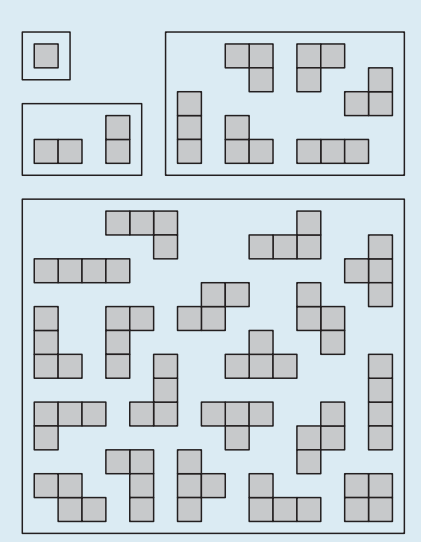
\includegraphics[width=0.6\textwidth]{polynominoes.png}
    \caption{The single monomino (A(1) = 1),
    the two dominoes (A(2) = 2), the A(3) = 6
    triominoes, and the A(4) = 19 tetrominoes
    (Tetris pieces) \cite{polyominoes}}  
\end{figure}
Tetrominoes are a special case of polyominoes (A(4)), which are shapes made up of squares. This is another interesting field of study, and a possible route to increase complexity in tetris, as the number of possible shapes increases dramatically as discussed in Barequet et al.\cite{polyominoes} and visualized in Figure \ref{fig:poly}.
This path however will not be followed in this project.
\paragraph{Mathematics}
There are few computer games whose mathematical properties have been research to the same degree as Tetrises. The following section will give a short but incomplete overview.
\subparagraph*{Tiling} is a funamental problem in mathematics. It deals with the problem of covering a plane with a set of geometric shapes. While this relates directly to the gamesplay, it has also found interes in scientific research such as robotics \cite{tiling1} or neuroscience \cite{tiling2}. While these articles do not require the existence of Tetris, it has certainly sparked intereset in the domain and helped with visualiing and understanding the problem.
\subparagraph*{Complexity - } One of the most renowned scientific papers in game-related computer science is a proof by Demaine et al. that Tetris is NP-complete \cite{tetris_np}. 
Beeing NP-complete means that Tetris is at least as hard as the hardest problems in NP, which are the problems that can be solved in polynomial time by a non-deterministic Turing machine. This means Tetris is one of the hardest problems in computer science.
\newline
\newline
While all this does not influence the development of our 4D Tetris variant, it does inspire how far such a simple game can grow. And there is a hope that a variant in a more complex space will intice similar research.

\paragraph{User Interface}
Part of the success of Tetris is its accessability. There is no need to explain anything. The main menu features a button named "Start" and the game is controlled. The game screen shows the playing field and the rest of the screen is used to display the next block, the score, the level and the lines cleared. 
There is no explanation needed. This is a feature that needs to be replicated to make the game accessible to a broad audience. The difficulty will be to translate the increased compelxity of this project into an accessable product.
\paragraph{Conclusion}
Tetris was a pivotal work. There is a reason it is displayed in the Museum of Modern Art in New York. It has inspired so many different fields and captured millions of players. This all needs to be kept in mind during developemtn as I want to capture a similar feeling of simplicity and complexity in our game.
\subsection{Frac 4D}
This is a game developed in the early 90's and never completed. It featured 4 distinct, but connected 3 dimensional playing fields. Pieces can be rotated and due to their underlying 4 dimensional structure this will reveal different configurations, the can exist in some of the fields but not in others, which can lead to unexpected 'collisions'. The game was apparently very hard to play and in the end failed to provide an easy access into 4 dimenesion.
\begin{figure}
    \label{fig:frac4d}
    \centering
    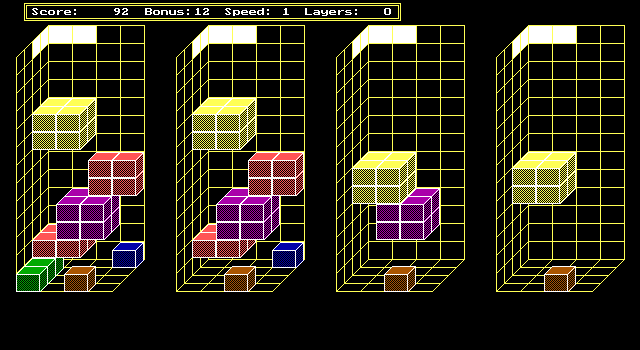
\includegraphics[width=0.6\textwidth]{frac4d.png}
    \caption{The 4 playing fields of Frac 4D. Image from myabandonware.com}
\end{figure}

\subparagraph*{Conclusion}
This game was probably the first 4D adaption of Tetris, and while featuring interesting concepts failed to succeed. There is however features that can be taken from this attempt, especially the highlighting of the corresponding position in the playing field to help the player as seen in Figure \ref{fig:frac4d}.
\subsection{4DTris}
This was another venture into the 4th dimension with Tetris. The concept however is completely different. This time the actual playing field exists in 4 dimensions and the pieces do as well. The playing field is projected into a hypercube, as are the pieces, which ends up looking at a cube the is beeing filled from the inside with different cubes. Development was stopped in 2012 and the author moved on, eventually trying to revive it in 2018, failing. The concept is very interesting, but very hard to imagine. While playing the game might make on proficient, the learning curve would be to steep for most.
\subparagraph*{Conclusion}
For me this is an example of a variant that went to far. While very intersting in concept, the sheer complexity of the gameplay automatically limits the addressable market. In this project falling into the same trap needs to be avoided by creating something fun for many different audiences.
\begin{figure}
    \label{fig:4dtris}
    \centering
    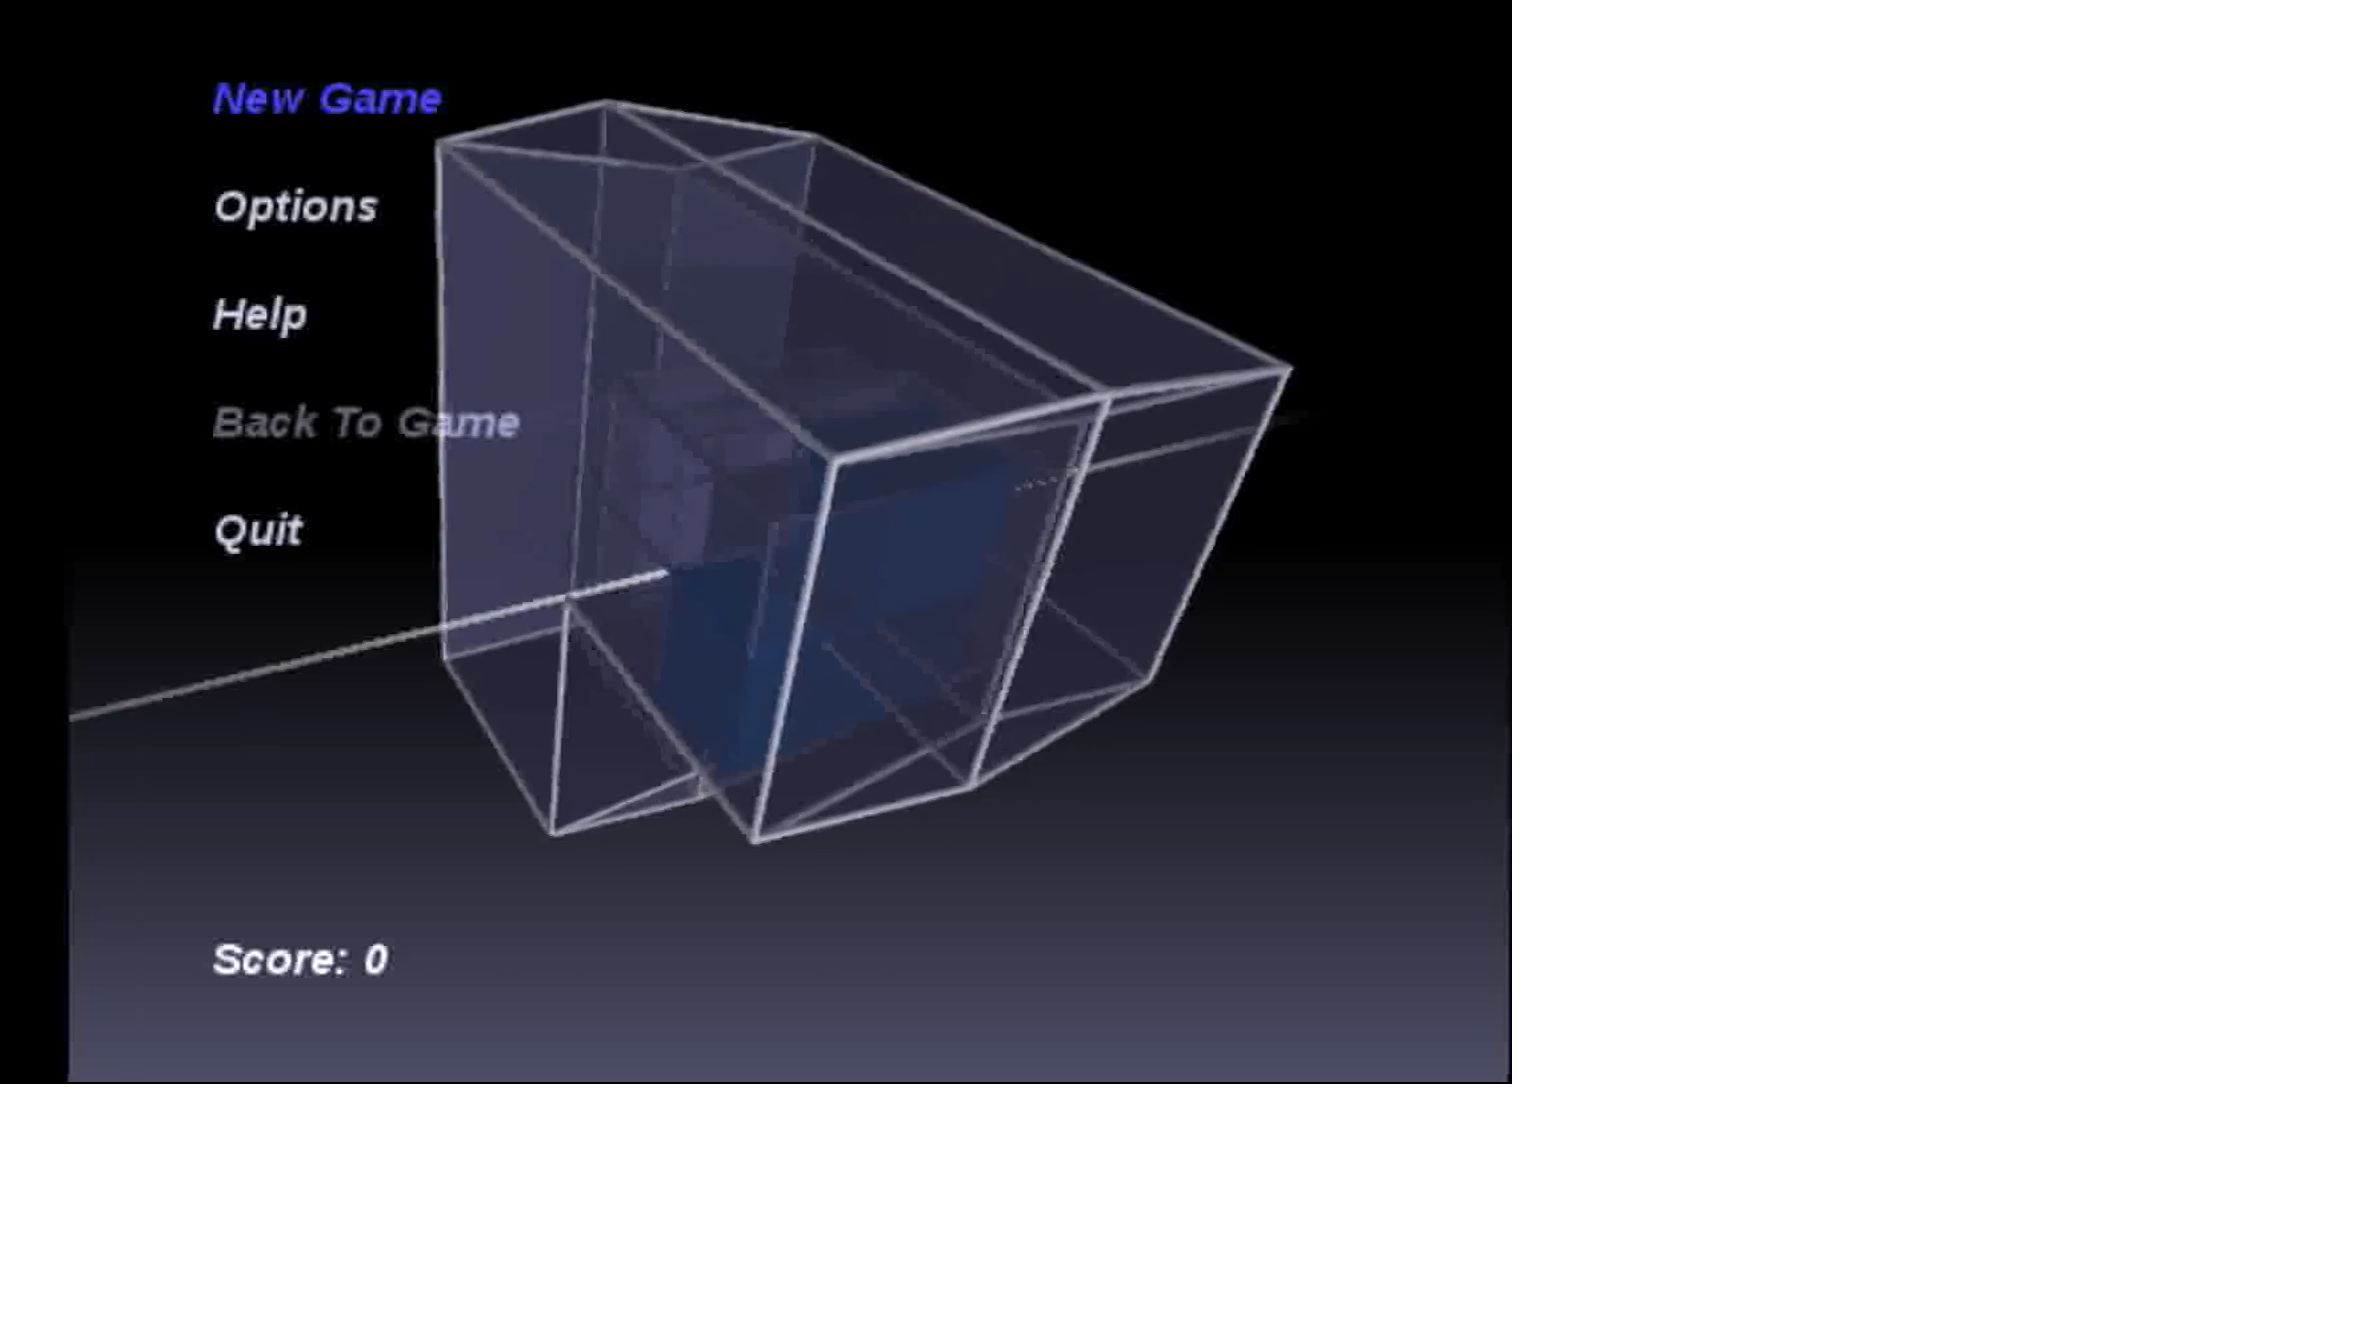
\includegraphics[width=0.6\textwidth]{4dtris.png}
    \caption{4DTris in action. Still from a video on youtube, posted by the autor Simon Laszlo, https://www.youtube.com/watch?v=WO9SNW5Tp7A}
\end{figure}
\subsection{BlockOut}
BlockOut is a 3D Tetris variant. The playing field is a 3D cube and the pieces are 3D shapes. 
The playing field is projected from above. Individual layers are color coded. In any other way the game is very similar to Tetris. The game was moderately successful and can be played online for free nowadays.
\subparagraph*{Conclusion}
This is a great example of a Tetris variant and something that my version will largely be based on. I want to take large parts of the visualization style but enhance on UI/UX.
\subsection{ TODO }


\subsection{This project}
will be an amalgamation of all the above. Taking the best features from every item. Looks from BlockOut, physics from 4DTris, UX features from Frac4D and general greatness from Tetris.

\section{Literature}
Understanding 4 dimensional space and its implications is a very challenging undertaking, however there is some literature out there that can help with the process. 

\subsection{The Fourth Dimension} by Rudy Rucker \cite{rucker} takes us through a wild journey from ancient mathematics to conteporary philosphy and the other way round. This can create great insights on how it is possible to understand and even visualize 4 dimensional object within reality that is confined to 3 dimensions. This work does greatly help with becoming comfortable with the concept of 4 dimensions and will be a great help in the development of the game.
\newline
While this is not comparable to peer reviewed literature in quality, it is a good read to deal with the difficulties of the topic. He touches on historical literature that deals with similar topics from Plato to the somewhat famous novel of Flatlands. Both deal with the perception we have of our dimensionality and how situations (Plato) or beeing a lower dimensional beeing (Flatlands) could change that perception. This helps open our minds to think about the 4th dimension. He also covers how we can represent the 4 dimensional object by slicing it with a 3d plane, without going into the mathematical aspect of it. 
The book helped me to visualize in my head on how i wanted my 4d interpretation of the game to look like.

\begin{figure}
    \label{fig:4d}
    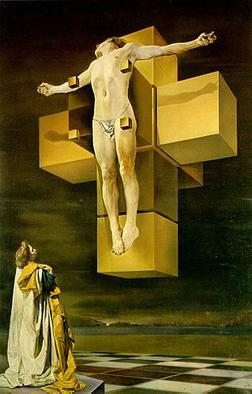
\includegraphics[width=0.6\textwidth]{Dali_Crucifixion_hypercube.jpg}
    \caption{The Crucifixion (Corpus Hypercubus) by Salvador Dali. A representation of a hypercube unfolded into 3 dimensions.}
\end{figure}

\subsection{Geometric algebra for computer science} by Leo Dorst, Daniel Fontijne and Stephen Mann \cite{geo_alg} serves as a great introduction into geometric algebra, which might be a solution to the problem of representing, and especially rotation 4 dimensional objects. The book explains how algebraic expression can be extented to geometric shapes, introduces the idea of multivectors, and how the are used to manipulate geometric objects. There is some coverage on how to implement the techniques used in code. Published by Morgan Kaufmann, this is not peer reviewed, but a commercial book. The authors are accredited academics, which should give the book some credibility.
\subsection{An Introduction to Clifford Algebras and Spinors} by Jayme Vaz Jr. and Roldao da Rocha Jr. \cite{cliff_alg} is another great resource into the topic, especially as Cliffor algebras are widely used in n-dimensional geometry. The chapter on spinors is especially interesting as they are one of the ways to represent rotations in higher dimensions.
The authors of this book are well known, and while this book is not peer reviewed it is published by Oxford University Press, a well known publisher of scientific literature.
In the end this turned out to be far to complex for this project, as I was able to approximate the rotations with a much simpler approach.

\subsection{On Rotations in Space of Four Dimensions} by Cole \cite{rot_n_1} is an article from 1888 that deals with the problem of rotations in 4 dimensions. The article proofs a general rotation matrix for 4 dimensions. The most important feature however is the date of publication, proving the persistent human interest in the topic of higher dimensions and therefore (somewhat) validating the project.
\newline
While beeing a very old article, it describes how to construct a 4x4 matrix from the rotations. In the end this was the technique used in this project, since it was simple but effective. being a peer review journal article, that has been cited often, I believe this to be a credible source of information.

\subsection{Conclusion}
This is just a small outtake on literature that can help understand the topic of higher dimensions which is necessary for this project. Especially the decision on which mathematical representation and technique will be chosen is heavily informed by these books/articles.

\section{Visualization}
Visualization of 4 dimensional objects is a very challenging but interesting task.

There is a large amount of great resources available to help understanding how this can be done. A very good overview over the techniques is presented in the PhD thesis by Hallasch \cite{4d_vis_1}. In extension to this the website "https://baileysnyder.com/interactive-4d/4d-cubes/" \cite{4d_vis_2} offers great interactive tools to generate an understanding of how to get to 4d dimensions and back.
This is again not a peer review source and any information gathered here should be questioned. However since it is a free resource, and the results did approximate my expecations, it did help me understand the topic better.
\subsection{Illuminating the fourth dimension} Illuminating the fourth dimension by Hanson et al. \cite{4d_vis_3} describes multiple techniques on how to render 4d objects into 3d space onto a 2d screen. This includes advanced shadowing and shading techniques which exceed the necessity of this project since unity will be used.
\newpage



\section{Domain and Users of the Project}
% Approximate Word Count: 300 words
\subsection{Gamers}
I will try to capture a wide audience for this game. 
Tetris is played by young and old, people from different educational backgrounds and different cultures.
As described by Csikszentmihalyi \cite{flow} this can be done by creating a state of flow. To induce this state several things must be true.
\begin{enumerate}
    \item A challenging activity that requires skill
    \item Clear goals and feedback
    \item The player must be able to concentrate on the task at hand
    \item Direct and immediate feedback
    \item A sense of control
    \item A loss of self-consciousness
    \item An altered sense of time
\end{enumerate}
When looking at this list, it is clear that Tetris succeeded in all of them. The biggest challenge for this project will be to make it easy enough so users of all backgrounds can achieve 'flow'. As Chen \cite{flow_2} stated this can be achieved, by unlocking additional choices (pieces) when the player has obtaines some suffiency. Some users will struggle with the basic concept of higher dimensions, and the game is required to ease them into a basic understanding of how the rotations work. Others will have no issues getting into the game but will require additional challanges to be sucked into the game and keep engaged. The game needs to create a sense of reward in users playing it for 5 minutes during a short break as well as users that are willing to invest several hours to achieve higher scores. Due to the nature of the game it is expected that it will have a somewhat larger appeal on users with advanced education, so these will be the primary focus group during evauation, however, previous projects into the same realm have shown that focussing solely on this group will not be enough to create a successful game. Targeted testing will be carried out, and I will try to include at least 25\% of the testers from a group with a lower educational background.
\newline
While these are the target audiences for the game we have to accomodate the fact the the main group of users will be male, between 20-40 years old and most likely with a higher educational background. This will be the primary target group and affect marketing and pricing strategies.
\subsection{Research}
A secondary target user group will be the academic community. Tetris has been widely used as a research subject. Our variant will rely heavily on mental rotation and spatial reasoning, both have been an important part of psychological reasearch \cite{COOPER197520} \cite{CORBALLIS1997100} \cite{Kornhaber_2020} \cite{Lau_zhu}. This could be a very interested target audience if the game itself implements features that aid researchers in experiment design. Voice of customer will be conducted in advance of development to gain insights into what specific features would be suitable to engange the scientific community.
This might be as simple as exporting pieces spawned + keystrokes into a csv file.
% Explain the domain (e.g., educational gaming) and describe the target users.

\section{Justification of Design Choices}
% Approximate Word Count: 350 words
Several choices had to be made during envisioning.
\subsection{4D}
While it was very enticing to try to implement a fully 4 dimensional game and or move tha play field into 4D as well. Preliminary user research as well as an extensive review of previous work has shown that this would increase the comlpexity to a level where the likelyhood of overall commercial success for such a project would decrease dramatically due to a decease in target users and the total obtainable market. I will therefore limit the playingfield to 3 dimensions and the pieces to 3 dimensional slices of 4 dimensional objects.
\subsection{Gameplay}
Due to limitations when it comes to user input the interactions within the 4th dimension will be limited. To be precise ther will be no way to move the w plane and change the slice we are prohecting into 3d space. The w plane will always be in the middle. This does however leave and opening for later expansion/enhancment of the gameplay.
\subsection{User Interface}
I feel that it is necessary to create a very informative user interface due to the complexity of the game and the fact that the arrow keys will have different functionalities depending on which action key is pressed. This shall be achieved through graphical overlays that will inform the player of the type of rotation/movement that will be performed in the current state.
\subsection{Scoring}
For the prototype multiline tetrises will be disabled. The primary goal of the MVP is to establish fun and engaing gameplay.
\subsection{Art Style}
The art style will be very important for the game. While people with higher educational background will likely be enticed by the mere concept of a 4 dimensional game, other user groups will need appealing and contemporary visuals to be kept enganged.


% Explain how your design decisions meet user needs and fulfill domain requirements.

\section{Overall Structure of the Project}
% Approximate Word Count: 350 words
The game will be made out of several components that will interact with each other. The main components are:
\subsection{GameManager}
This will take care of the overall game state. It will keep track of the current score, the current level, the current piece, the next piece, the playing field and the current state of the game. 
\subsection{HyperCube}
The basic building block of the game. This will be a 4 dimensional extension of a cube. It will be used to procedurally generate the mesh userd for rendering the pieces as well as basic rotation logic. Collision detection will be done in 3 dimensional space.
\subsection{Piece}
This will be a 4 dimensional collection of hypercubes. the main rotational logice be implemented here. The current plan is to decimpose the piece once it is resting on the playing field. In addition the rendering will switch from wireframe to solid. With individual cubes rendered in a color accorading to the row they are on.
\subsection{Block}
This will be the collection of all resting cubes and will be used for the detection of completed planes.
\subsection{Level}
This is the playing field. Will generate the mesh, keep track of the block and give options for later enlargement of the playing field (not in MVP).
\subsection{User Interface}
Will be a column on the right containing scores, level etc. as well as an overlay that will help the user understand the rotations.
The main plan to achieve this is to have a graphic that represents the arrow keys. Whenever one of the modifier keys is pressed the text, and maybe the colour of these arrow keys will change to give the player an idea of what rotational plane will happen. The problem lies in the actual rotations changing depending on the starting rotation. It might be necessary to have a visualisation of the current pieces somewhere in the UI that represents all 4 possible rotations with the current modifier, this could be turned off at a later stage (difficulty). Since this is one of the main challenges other preceding games have faced, this needs to be an area of focus and further testing. 
\subsection{InputManager}
Will switch between different state depending on the action key pressed changing the functionality of the arrow keys and relaying the information to the pieces.
\subsection{AudioManager}
Will take care of the audio. Will be very basic in the MVP.

% Describe the architecture, including main components and their interactions.

% Include diagrams (not counted in word limit).
\begin{figure}[H]
    \centering
    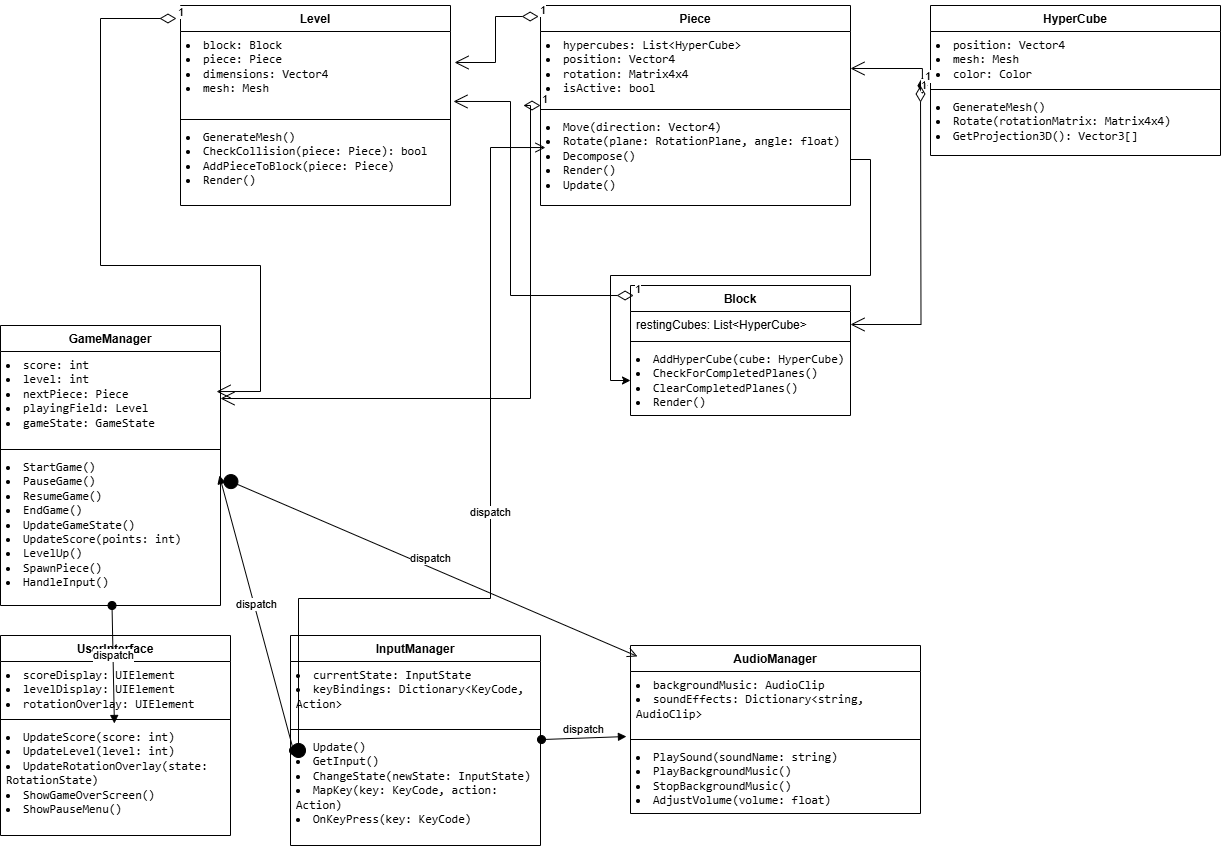
\includegraphics[width=\textwidth]{classes.png}
    \caption{Overall Architecture of the 4D Tetris Project}
    \label{fig:architecture}
\end{figure}

\section{Important Technologies and Methods}
% Approximate Word Count: 300 words
\subsection{Unity} is a requirement of the course. We will use the powerful game engine to handle everything from rendering, through audio for us. It is of yet undecided if the built in physics, collision and math modules are sufficient for this project or will need to be implemented.
\subsection{C\#} is an object oriented programming language that abstracts away a lot of the details one has to deal with in lower level leanguages such as C++ and adds garbage collection. The downside is less fine detail control.


\section{Plan of Work}
% Approximate Word Count: 250 words

The Main activity in developing the project are going to be testing and developing. The additional task of writing the report will be done in parallel throughout the development. The most important features are outlined in the following Gantt chart, with ample amount of time included for unexpected challanges.
In addition, due to a full time job, weeks that require business travel are included as well, as it is highly unlikely that any development can happen during those times.

\begin{figure}[H]
    \centering
    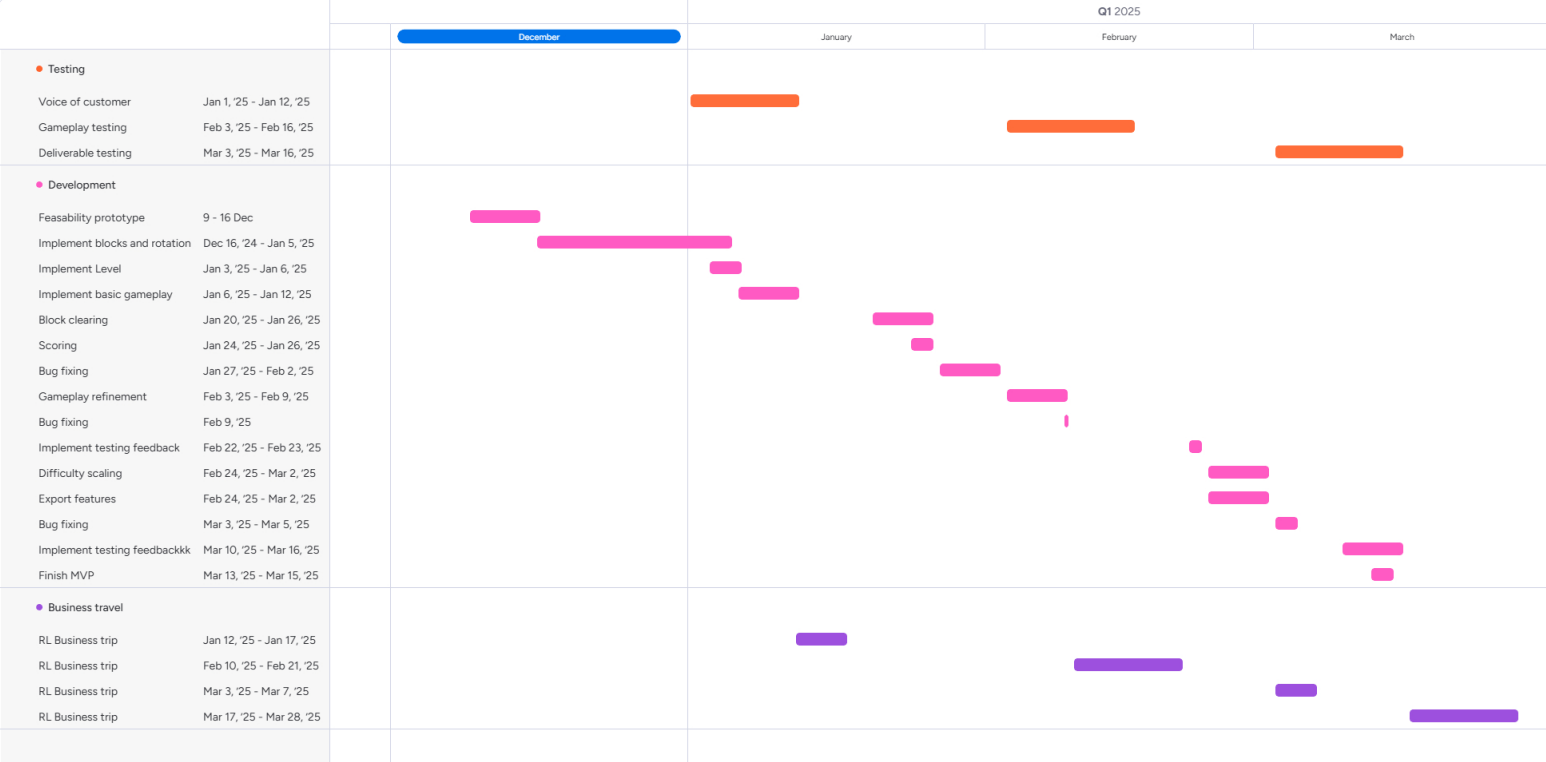
\includegraphics[width=\textwidth]{gantt.png}
    \caption{Project Timeline Gantt Chart}
    \label{fig:gantt}
\end{figure}

\section{Testing and Evaluation Plan}
% Approximate Word Count: 250 words
Recurring Testing is key to a successful completion of this project. Given the limited time available for development there will be a total of 3 main test phases.
\begin{enumerate}
    \item \textbf{Voice of customer} - This primary testing phase will not test the actual software, but the assumptions I have taken so far. This is meant to inform me on different aspects before starting the development phase:
            \begin{enumerate}
                \item Is the idea interesting
                \item Are the keybindings to complicated
                \item Is the chosen graphical style appropriate 
                \item Does the concept sound interesting
                \item How would you like level progression to go
                \begin{enumerate}
                    \item faster speed
                    \item more complicated pieces
                    \item ...
                \end{enumerate}
            \end{enumerate}
    \item \textbf{Gameplay testing} - After having created a feasible prototype, most likelz with limited audiovisual appeal. We will try to get some information from the users whether the gameplay eorks.
            \begin{enumerate}
                \item Do you understand what you have to Do
                \item Do you understand the basic visuals
                \item Are you aware how to line up the pieces
                \item Is the speed ok
                \item Is the point system rewarding
            \end{enumerate}
            In addition we will have some UX/UI related questions
    \item \textbf{Deliverable testing} - This final testing run will be used to test if the deliverable is up to spec. I will use the 'outstanding' criteria in the template as a reference and get metrics on how close we are to that goal. In addition users will be asked to rate different features of the game on a scale from 0 to 5 to identify any outliers. The goal is not to reach 5 in every categorz, but to identify components that perform below the average of the game. These might include:
            \begin{enumerate}
                \item Visual appeal
                \item Audio effects
                \item enjoyability
                \item Difficulty
                \item complexity
                \item Ease of use (UI)
            \end{enumerate}

    
\end{enumerate}

\section{Prototype}
\paragraph{Description}
Prototyping will go through several stages. Some are performed in Python, to quickly check my reasoning. Other features will be tested in Unity directly.
\paragraph{Rotations}
The first feasibility issue was the rotation of the 4 dimensional pieces and the projections into 3D space. To check if I was able to generate the correct roations and the vertices I implemented a very basic símulation in Python. The reasoning
behind this was, that Python support higher dimensional matrices out of the box and it seemed like a fast approach. In this round of prototyping I was able to show that I am able to produce the rotations as well as the projection, and in addition+
that the rotation of the pieces looks interesting and can lead to unexpected piece configurations just as planned.
\paragraph{Basic movement}
Basic movement prototyping was done in unity to learn how to simulate the tetris style movement of 1 tile per button press, but gradually interpolate the position of the pieces.
In addition rotation of 4d hypercubes was also implemented in Unity to check general feasibility.
\paragraph{Conclusion}
While the prototypes are very rough, and not as far progessed as hoped to due to time constraints, they do show that the underlying concept is feasible and the project can be attempted. It did also inform me about important watchouts for the development phase, such as handling disconnected edges/vertices. Since in between rotations we return to 3D space, things like collisions and line clearing will be much easier to implement.

\section{Implementation}
\paragraph{Hypercubes}
\begin{figure}
    \label{fig:hypercube}
    \centering
    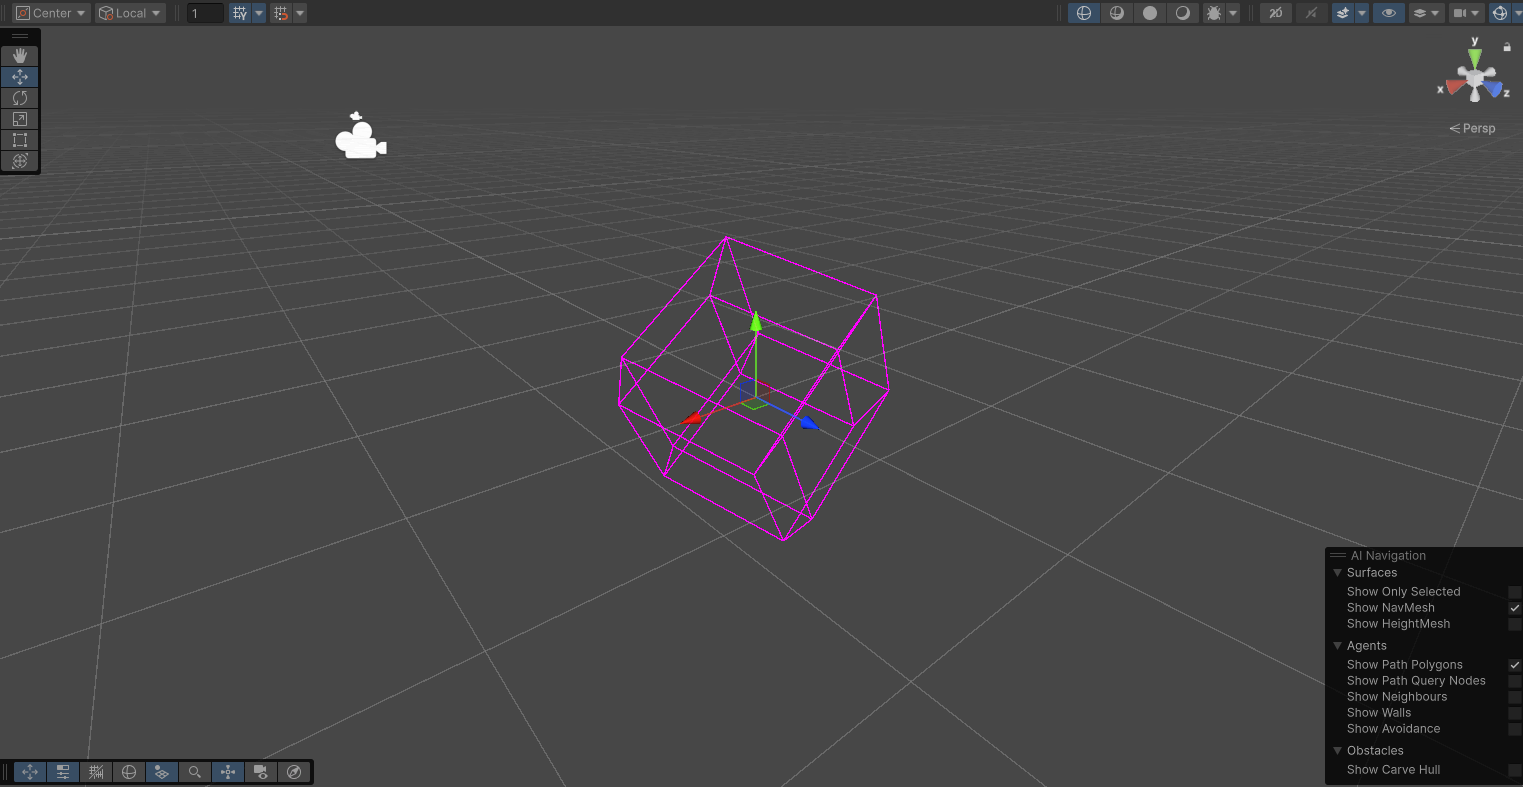
\includegraphics[width=0.6\textwidth]{./Dev/HyperCube1.png}
    \caption{A 4D hypercube projected into 3D space in Unity.}
\end{figure}
These are the basic building blocks of my game. It was the first module that was implemented. All the hypercube class does is instantiate 
The first thing this class does is create the vertices of the hypercube. This is done through 4 nested for loops that store 4 dimensional vectors in a list. 
From the vertices we can create the edges, a special property of 4d hypercubes is that two vertices form an edge if and only if they differ in exactly one coordinate. Since this is done only once on startup it is also implelented thorugh nested for loops.
\begin{verbatim}
    for (int i = 0; i < baseVertices.Length; i++)
    {
        for (int j = i + 1; j < baseVertices.Length; j++)
        {
            Vector4 vi = baseVertices[i];
            Vector4 vj = baseVertices[j];

            // Count how many coordinates differ
            int diffCount = 0;
            if (Mathf.Abs(vi.x - vj.x) > 0.001f) diffCount++;
            if (Mathf.Abs(vi.y - vj.y) > 0.001f) diffCount++;
            if (Mathf.Abs(vi.z - vj.z) > 0.001f) diffCount++;
            if (Mathf.Abs(vi.w - vj.w) > 0.001f) diffCount++;

            if (diffCount == 1)
            {
                edges.Add(new int[] { i, j });
            }
        }
    }
\end{verbatim}
To make the system easier, edges are not recalculated, but stay connected to the same vertices through the whole play. During inital testing this has not produced any critical issues, but might need to change in the future.
The Hypercubes are also in charge of creating their own mesh. For now we rely on a wireframe mesh, but this is still planned to change in the future. We simply store the current position of the vertices in a list and reference them in the index array. From this we create a new mesh each update (there is a lot of room for optimization here). This is necessary since we are not simply creating an object in 3D space, but we are rotating in 4 dimensions and create a different 3D cut each update, in addition we a interpolating the rotations to make the movement look smooth..
To obtain the positions of the vertices we use a helper class 
\begin{verbatim}
    public static Vector4 MultiplyPoint4x4(this Matrix4x4 m, Vector4 v)
{
    Vector4 result;
    result.x = m.m00 * v.x + m.m01 * v.y + m.m02 * v.z + m.m03 * v.w;
    result.y = m.m10 * v.x + m.m11 * v.y + m.m12 * v.z + m.m13 * v.w;
    result.z = m.m20 * v.x + m.m21 * v.y + m.m22 * v.z + m.m23 * v.w;
    result.w = m.m30 * v.x + m.m31 * v.y + m.m32 * v.z + m.m33 * v.w;
    return result;
}
\end{verbatim}
that lets us easily rotate a point by using a rotation matrix. Then we use a very trivial orthographic projection of the 4D space into 3D space. This is done by simply ignoring the w coordinate. This is a very simple approach, but it is sufficient for the current state of the project, an still gives nice visuals and interesting rotations. Future testing might compare a mathematically more correct approach against this in some sort of AB testing.
\paragraph{Polynominoes}
This module  handles the actual pieces. It randomly picks from a list of pre-created polynominoe layouts and creates the necessary hypercubes as well as rotates the piece into a random (snapped to 90°) state. The class also handles the rotations of the polynominoe. Every frame we interpolate
between the current position and rotation as well as the target position an rotation. This is fortunately all baked into C\#.
\begin{verbatim}
    // Interpolate between current and target position
transform.position = Vector3.Lerp(transform.position, targetPosition, Time.deltaTime * 2);

// Interpolate between current and target rotation
for (int i = 0; i < 6; i++)
{
    currentRotation[i] = Mathf.Lerp(currentRotation[i], targetRotation[i], Time.deltaTime * 2);
}
\end{verbatim}
This provides us with smooth movements.
This class has seen some revisions already, especially when in comes to collision detection.
The first plan was to use the built in Unity collision detection system. I created a cube on top of every hypercube and attached a rigidbody to act as a collider and have constant collision detection. After thinking about it however, I discovered this would be quite wasteful, and instead we keep track of the extends of the playing field and the the location of all walls and all blocks, and every time the player ask for any kind of movement we query if the final positon after that move, not the interpolated one, is even possible. If not, in case of a wall we simply ignore the move, in case of a block that prevents further falling, we start a timer, that unless the situation is resolved, will lock the piece in place.
For now this does not consider the edge case, where a rotation leads to an out of bounds situation, which is however planned to be mitigated in the future.

Locking in place will not be handles by the polynomino. Instead it will hand itself of to the board, and be dissassembled.


\paragraph{Input manager}
This class handles all the input provided by the player. For this assignement the input is very limited as we are bound to the arrow keys, plus 3 modifiers. The chosen layout table is below:
\begin{table}[H]
    \centering
    \begin{tabular}{|c|c|c|c|c|}
    \hline
    Modifier & LEFT & UP & RIGHT& DOWN\\
    \hline
     & Move left & Move up & Move right & Move down\\
    A & XY- & XZ+ & XY+ & XZ-\\
    S & XW- & YZ+ & XW+ & YZ-\\
    D & YW- & ZW+ & YW+ & ZW-\\
    \hline
    \end{tabular}
    \caption{Input Layout: The arrow keys are used to move the piece, the A, S, D keys are used to modify the plane of rotation.}
    \label{tab:input}
\end{table}
To make it easier for the user to understand, for the moment a text field on the UI layer is updated whenever a modifier is pressed to inform the user what planes of rotation are currently beeing used. In the future this will be modified to a graphical overlay.
For the moment this class also handles the pieces falling towards the bottom, however this is not properly decoupled and will be moved in the future.
\begin{figure}
    \centering
    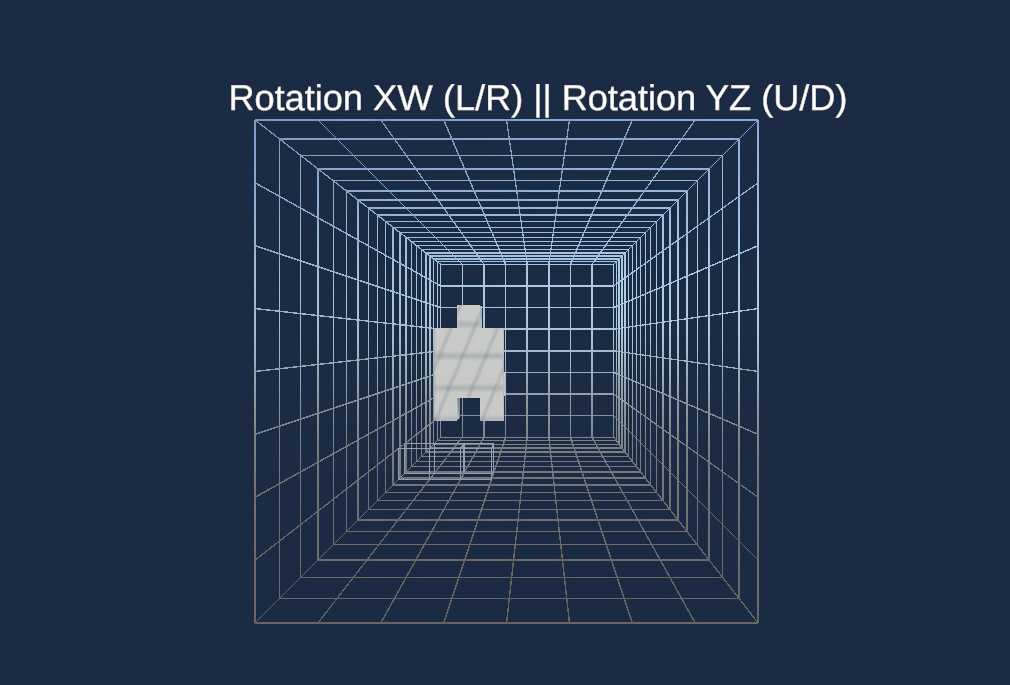
\includegraphics[width=0.6\textwidth]{./Dev/play_with_pointers.png}
    \caption{The current playfield with info about rotation (A key held down).}
    \label{fig:input}
\end{figure}


\paragraph{BoardState}
This class gathers information about the cells on the board. It is made up of a List of arrays of structs, that hold coordinates, a state and a cube. The Board State class provides crucial functions to other parts of the program such as Checking the bounds and checking for other pieces.
\begin{verbatim}
    public bool CheckNextFree(Vector3 targetPosition)
    {
        int x = (int)Math.Round(targetPosition.x) + (int)(GetBoardExtends().x / 2);
        int y = (int)Math.Round(targetPosition.y) + (int)(GetBoardExtends().y / 2);
        int z = (int)Math.Floor(targetPosition.z);
        if (board[z].cells[x, y].state == CellState.Filled)
        {
            return false;
        }
        return true;
    }
\end{verbatim}
This functions simply checks if a cell is already taken. Since we have discrete movements from cell to cell, even thoug we interpolate for graphical reasons, this is a much cheaper approach than doing acual collision detection or other complex techniques (could also raycast in z etc...).
This approach leads to appropriate stacking of the pieces.
\begin{figure}
    \centering
    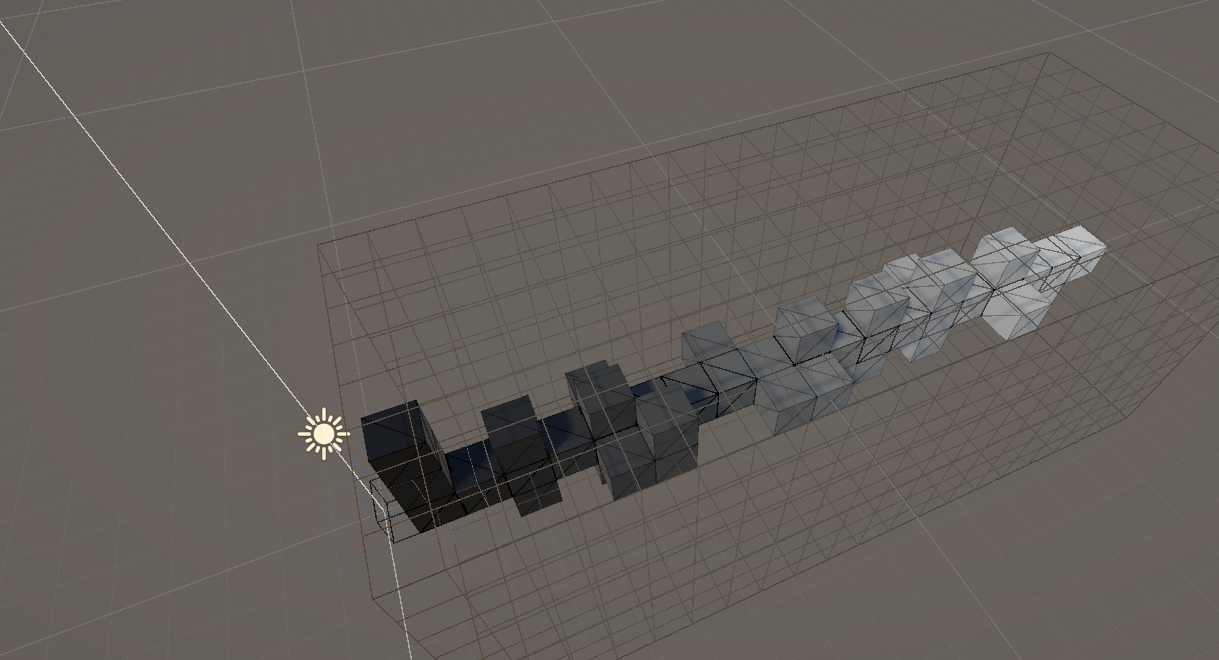
\includegraphics[width=0.6\textwidth]{./Dev/pieces piling up.png}
    \caption{Pieces stacking.}
    \label{fig:board}
\end{figure}
An even more trivial approach was chosen to check for the bottom. We simply check the Z coordinate an fix it in place.
\begin{figure}
    \label{fig:bottom}
    \centering
    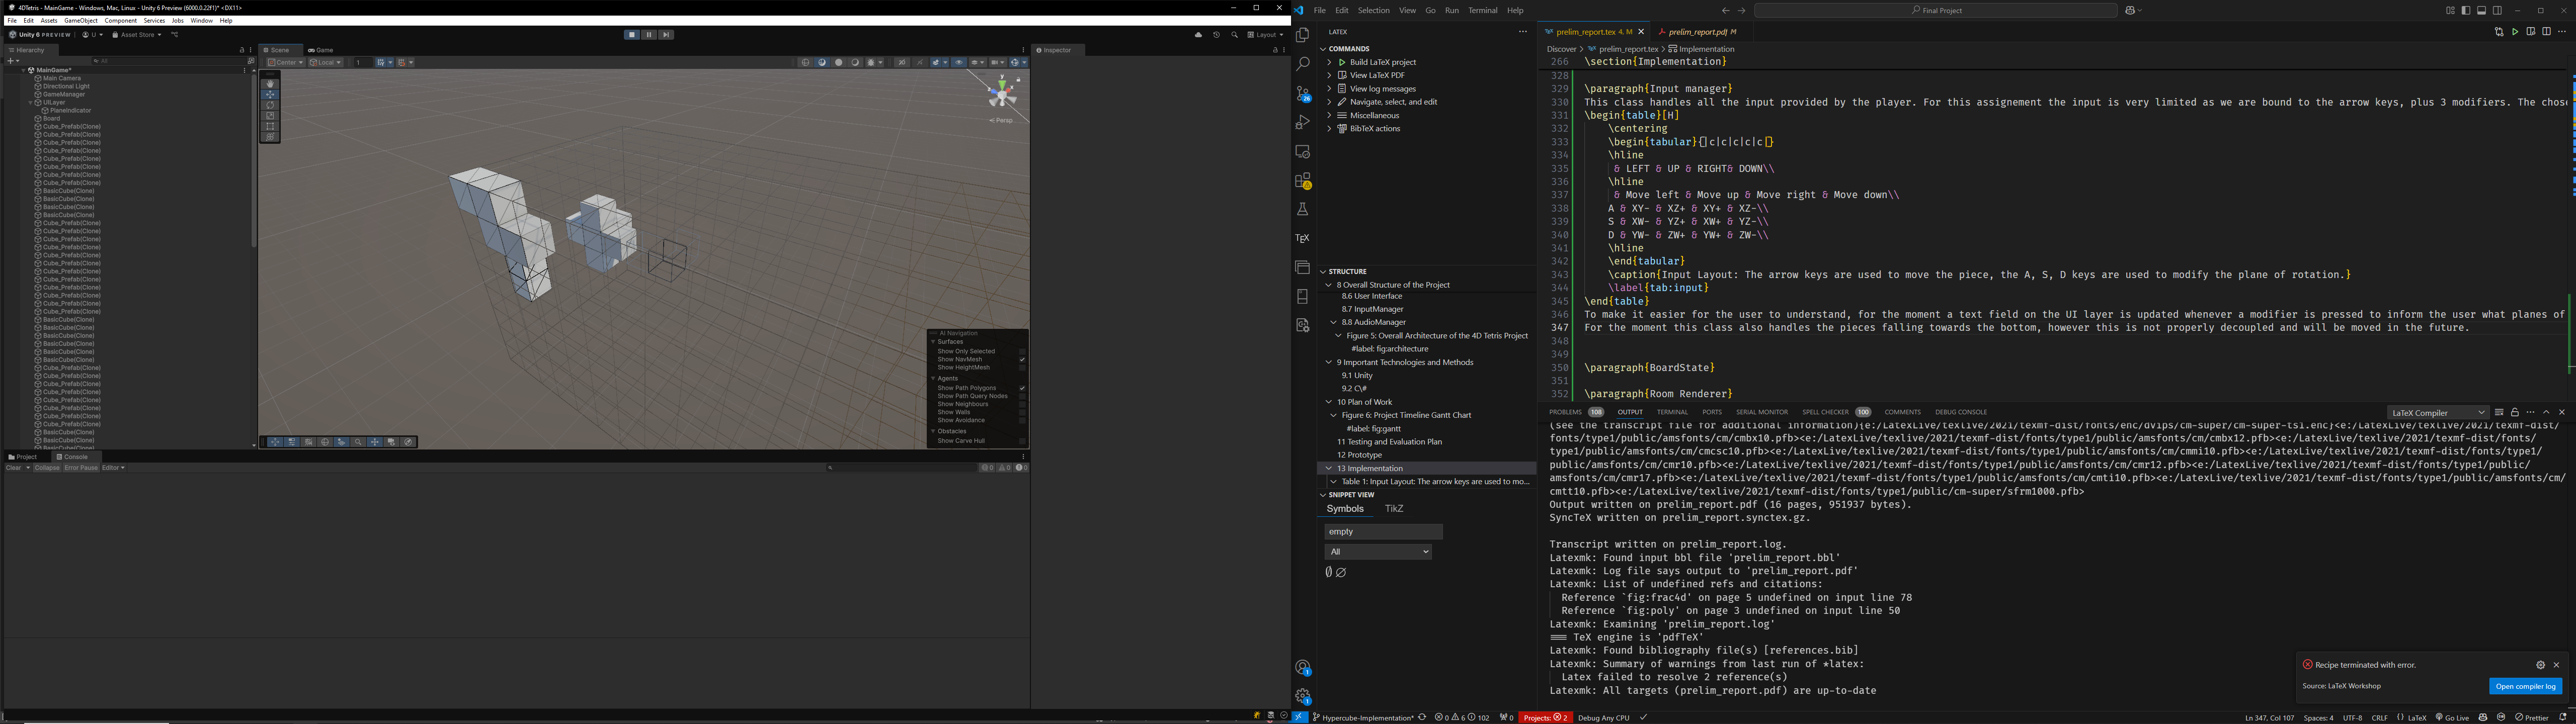
\includegraphics[width=0.6\textwidth]{./Dev/bottom working.png}
    \caption{Piece locked in place at the bottom.}
\end{figure}
The locking mechanism itself is done by removing the polynomino from the game and instanciating cubes in the grid, this also removes a lot of complexity.
\begin{verbatim}
    public void TransferCubes(Polynomino4D polynomino)
    {
        // Check the hypercubes of the polynominoe, calculate the position in the board grid and set it to filled
        foreach (var cube in polynomino.hypercubes)
        {
            Vector3 pos = cube.GetPosition3D() + polynomino.transform.position;
            int x = (int)Math.Round(pos.x) + (int)(GetBoardExtends().x / 2);
            int y = (int)Math.Round(pos.y) + (int)(GetBoardExtends().y / 2);
            int z = (int)Math.Floor(pos.z);
            board[z].cells[x, y].state = CellState.Filled;
 
            // Create a cube from the basic cube prefab and set it to this position
            Vector3 pos3 = new Vector3(x - (int)(GetBoardExtends().x / 2), y - (int)(GetBoardExtends().x / 2), z + 1);
            GameObject go = Instantiate(basicCube, pos3, Quaternion.identity);
            go.transform.localScale = new Vector3(polynomino.cubeSize, polynomino.cubeSize, polynomino.cubeSize);
            board[z].cells[x, y].cube = go;
            // Assign color based on z heioght
            float color = (float)z / (float)roomRenderer.sizeZ;
            go.GetComponent<MeshRenderer>().material.color = new Color(color, color, color);
 
        }
        Destroy(polynomino.gameObject);
        GameObject.Find("GameManager").GetComponent<PolyManager>().SpawnNewPolynomino();
    }
\end{verbatim}
To make it easier to indentify layers we color each cube in a layer the same color. The colors differ by layer and are assigned randomly at creation time of the board.


\paragraph{Room Renderer}
This class simply defines the size of the playing field and, for now renders a wireframe as seen in \ref{fig:input}. It also checkes the board for falling cubes and instantiates rectangles in all four side walls. This help to identify the shape of the object 

\paragraph{PolyManager}
Manages the spawning of new polynominoes. 

\paragraph{Conclusion}
The first 'sprint' was a somewhat enlightening experience. As the good saying goes, no plan survives first contact with the enemy. 
In this instance the enemy was my day job that suddenly required extensive overseas travel, which derailed my plan. But we had accounted for some travel, so the consequences can be somehwat mitigated. 
Another good learning experience was, that in nearly all circumstances my first solution was not the correct or best solution (nor are my current ones), but iterating over each function multiple times lead to much more elegant and efficient solutions. 
I feel that i am still in scope for what i tried to achieve in my project outline, but the 4D aspect, at least visually, will need some more work. 
Functionally we have a prototype that spawns random pieces, lets them fall down the board, they collide with the floor as well as other pieces and lock in place. Clearing is partially implemented. Once that is done, everything will be refactored. When looking back at the module that dealt with software decoupling I do recognise it in a lot of places in my own code and will want to clean that up before final submission.
Currently little unit testing has been done, this is mainly due to the fact that I was still figuring out the 'how' and unit testing without knowing the actual inputs and outputs that are required is somewhat futile. This will be done during refactor.
The visuals will also need a major overhaul, but this is planned for the next sprint.
Overall I feel confident that the project will be completed in time and to a satisfactory level. The main challenge is that I identified is playtesting, as the speed and the size of the board need to align with the limited time of 3 minutes that are available for the prototype.



\section{Evaluation}
\paragraph{Voice of Customer}
This was described in a former paragraph. The goal was to identify the actual need for such a game, and learn about general properties. This was done using a simple questionaire at a (local) university (faculty + students).
Some results can be seen in figure \ref{fig:voc}. What this shows it that there is a general interest in the game. The proposed keybindings (see table \ref{tab:input}) were liked, however I doubt that the results will be identical after playtesting.
The progession system was in most cases wanted as the normal 'get faster' approach, since this is not critical for the prototype in this module it will be left for later.
The question about the graphics was a little ambigous, since there was no concept art provided to the testees, this should be considered in future works.
\begin{figure}
    \centering
    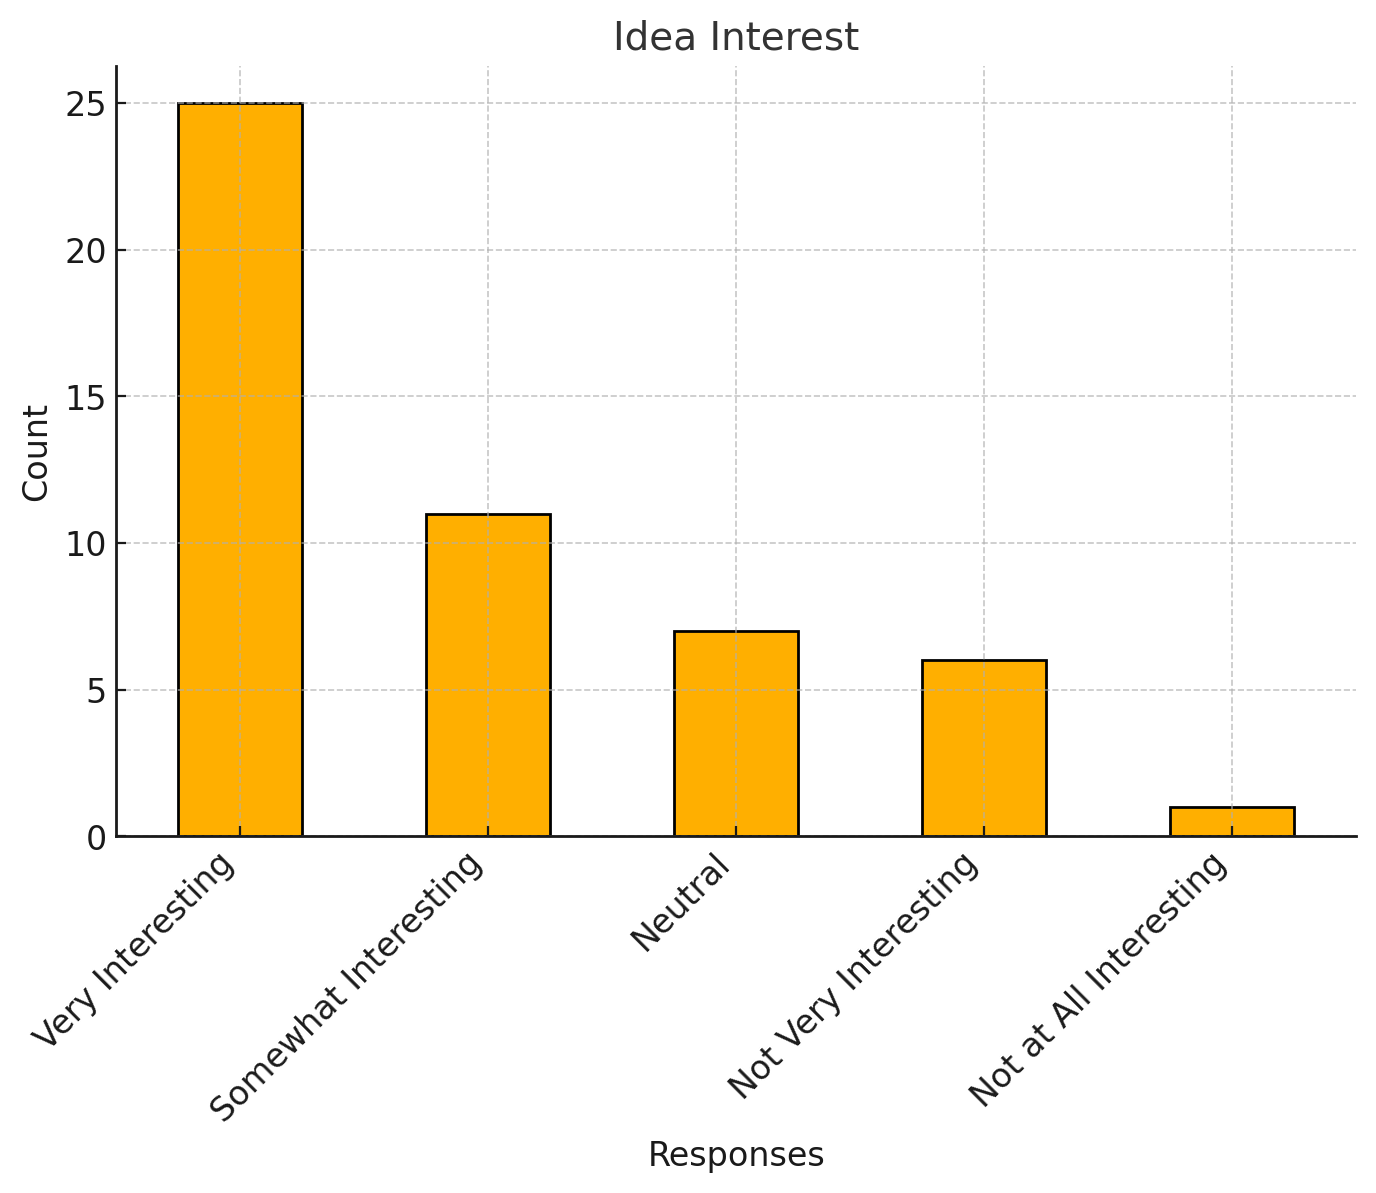
\includegraphics[width=0.3\textwidth]{./Dev/voc1.png}
    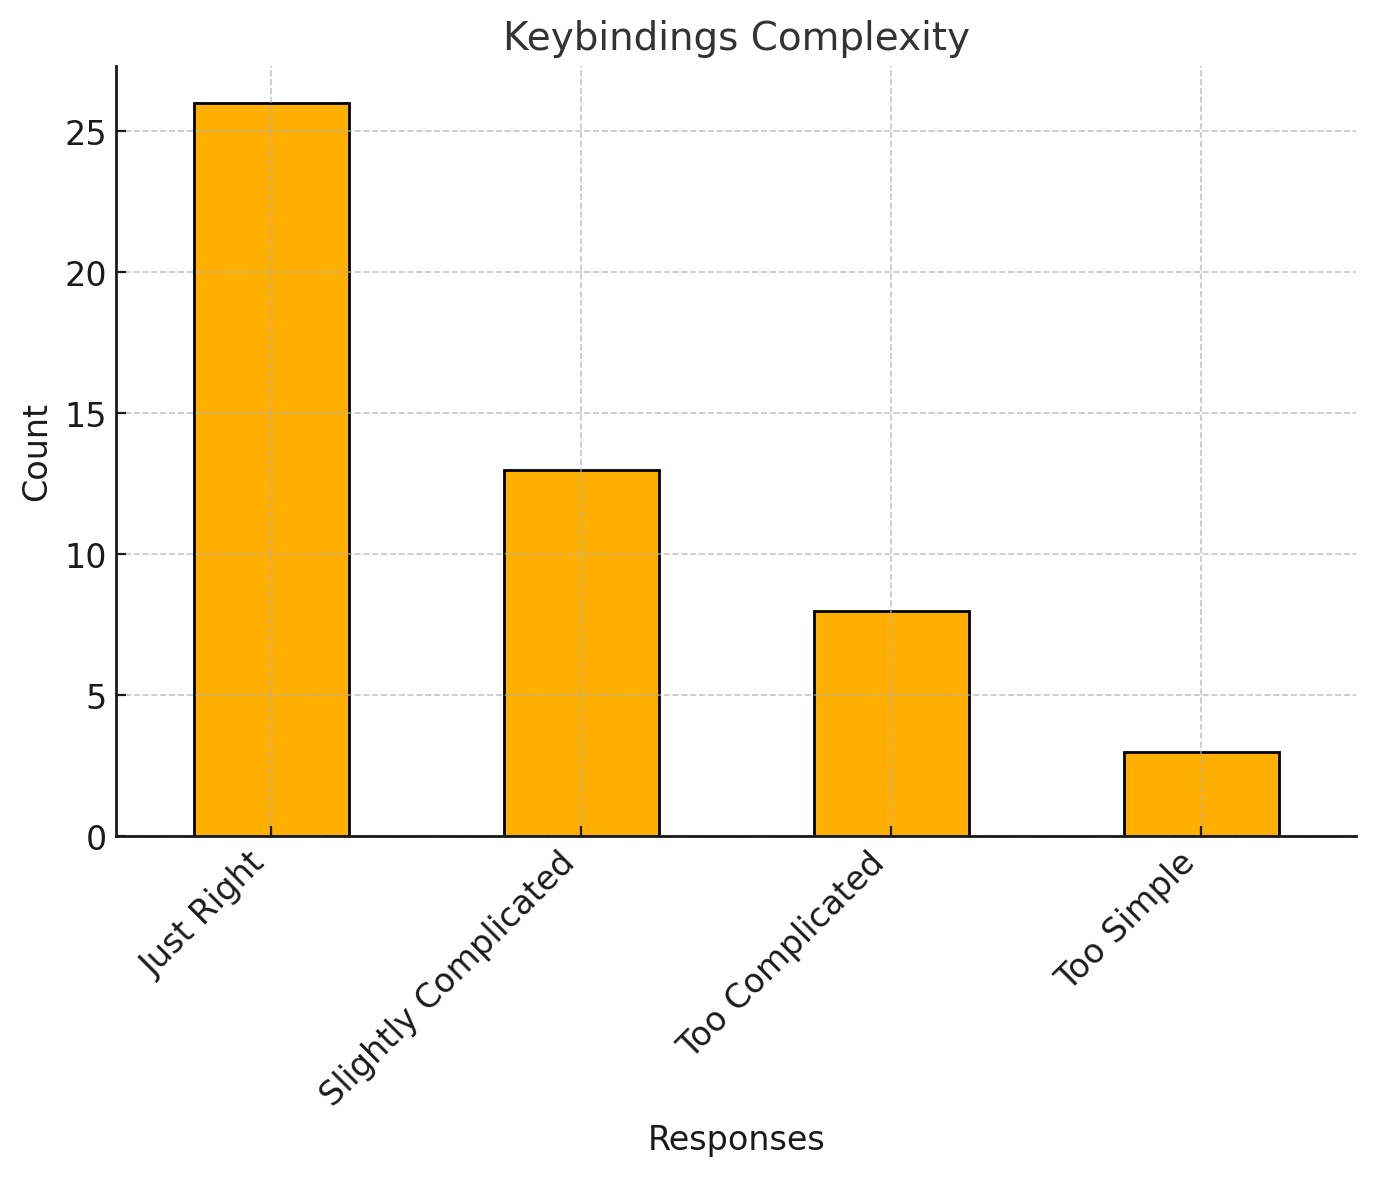
\includegraphics[width=0.3\textwidth]{./Dev/voc2.png}
    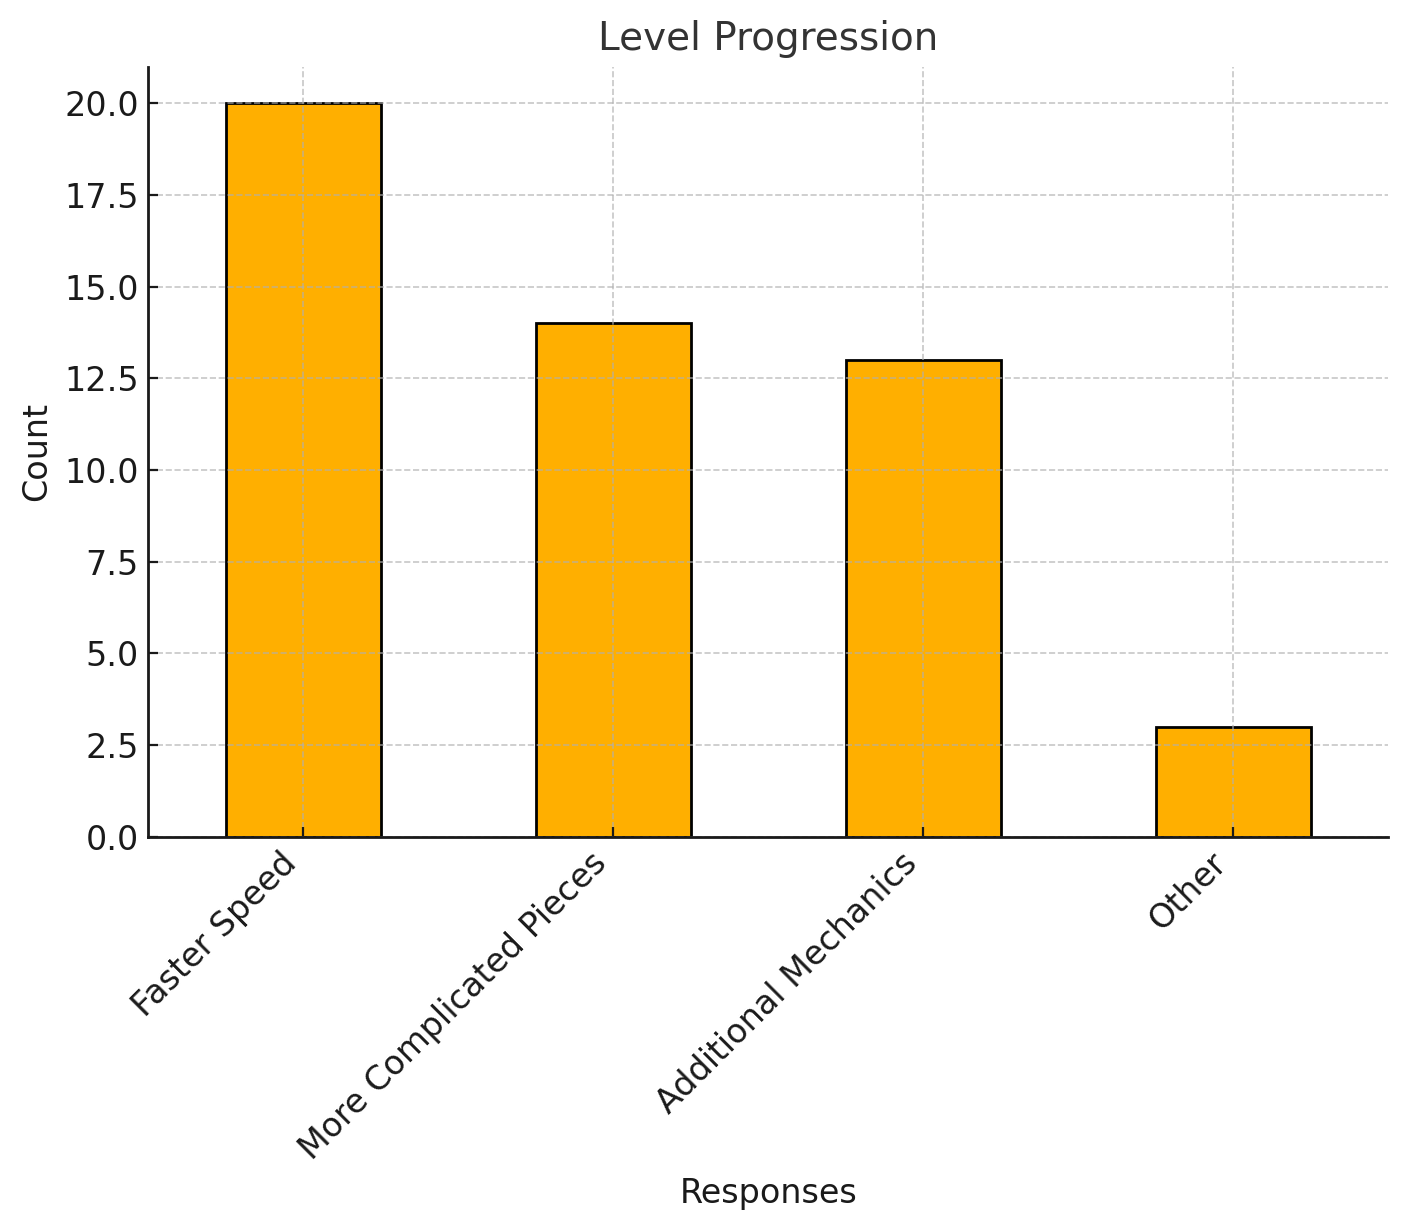
\includegraphics[width=0.3\textwidth]{./Dev/voc3.png}
    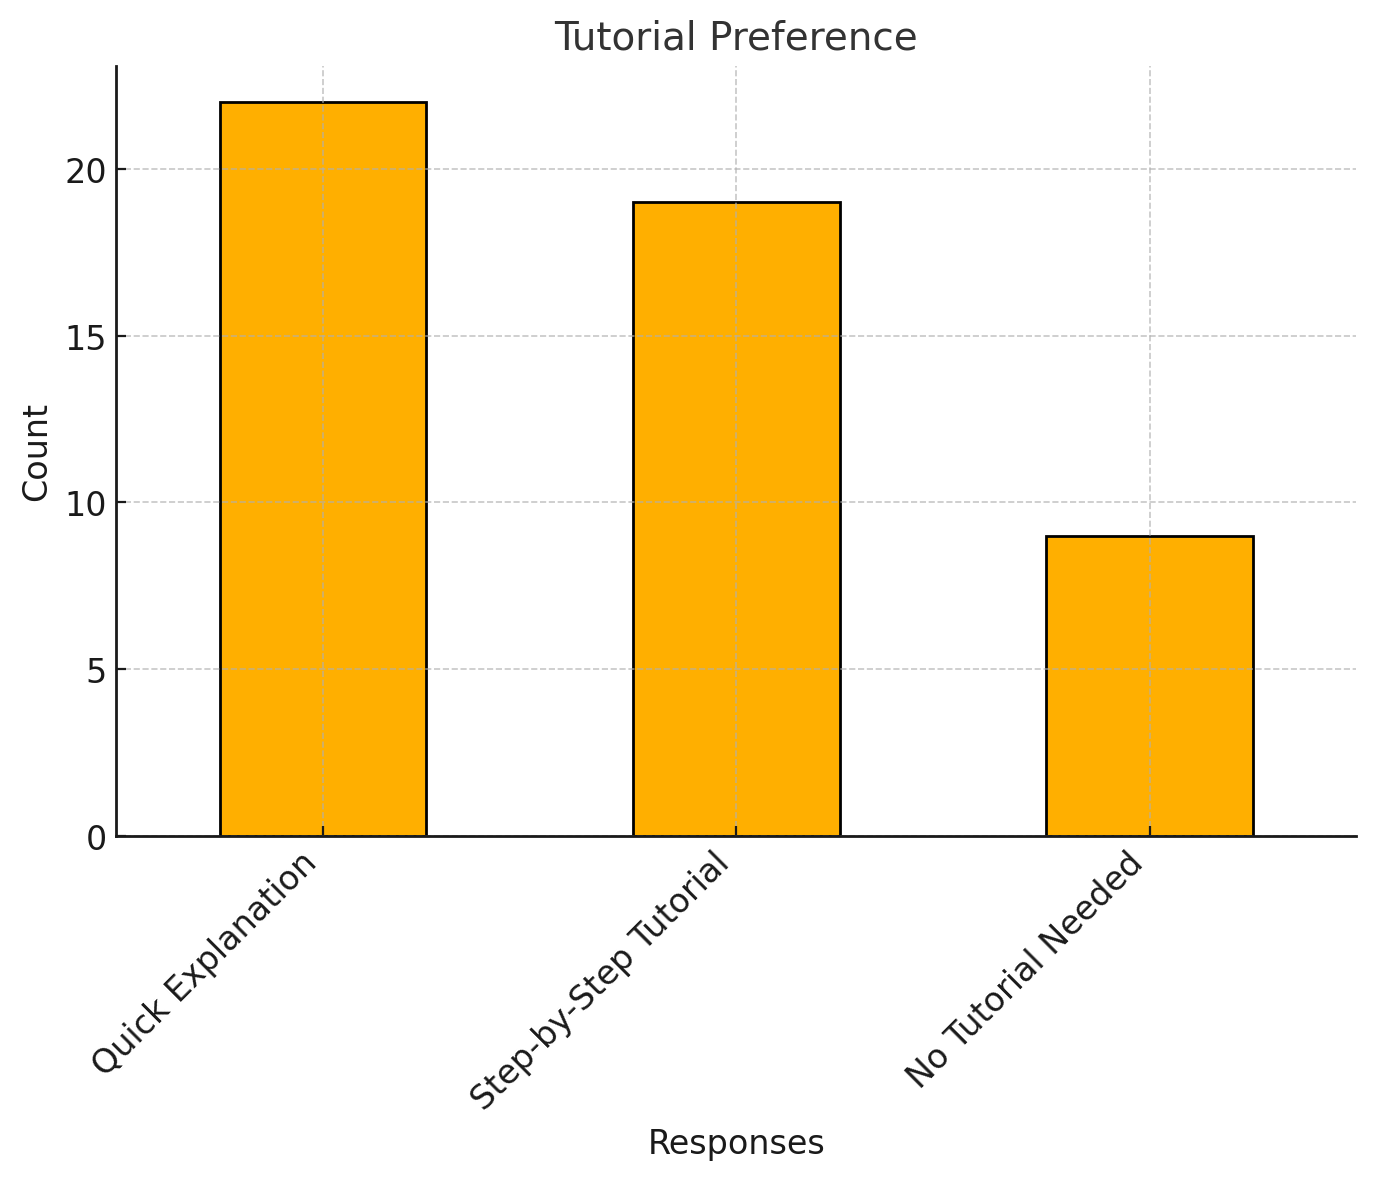
\includegraphics[width=0.3\textwidth]{./Dev/voc4.png}
    \caption{Results of the Voice of Customer Survey.}
    \label{fig:voc}
\end{figure}
\paragraph{Prototype Testing}
This test was renamed from Gameplay testing, since due to time constraints, some functions were not provided (score system).
This was performed in person on 10 people. The participants were betwenn 29 and 47 years old, and with a higher educational background, this needs to be considered, but more testing was not possible due to time constraints.\newline
The participants reveived a quick verbal intro the game concept. They were then left alone with the protype and asked to talk about visuals, the controls, game speeds, concept and general feedback.
Some key results are:
\begin{enumerate}
    \item Visuals are ok, multiple people want shading on the polynominoes
    \item Controls are fine, more guidance on what will happen during rotations would help
    \item Game feels slow
    \item Concept it interesting, the idea of 4 dimensional tetris pieces is hard to understand, for a full release an actual physics intro would be fun
\end{enumerate}
This second round of user testing was very informal, but very informative. Having people playing it live and giving direct verbal feedback provided me with many ideas how to inprove in the future.

\paragraph{Unit testing}
As mentioned above, this was not yet done. Due to my own lack of understanding how to solve the problems it felt constructed to unit test, and I was unaware of many of the actual edge cases. The plan is to do user testing during the refactor, since i now know how it can work, and will work on optimizaztion and decoupling this could be a good place for unit testing.

\paragraph{Gameplay testing}
Gameplay testing was done during the final week of development, with simultanous bug-fixing. The target audience consisted of 5 people, again all with academic background, but different previous exposure to video game. 
\begin{figure}
    \centering
    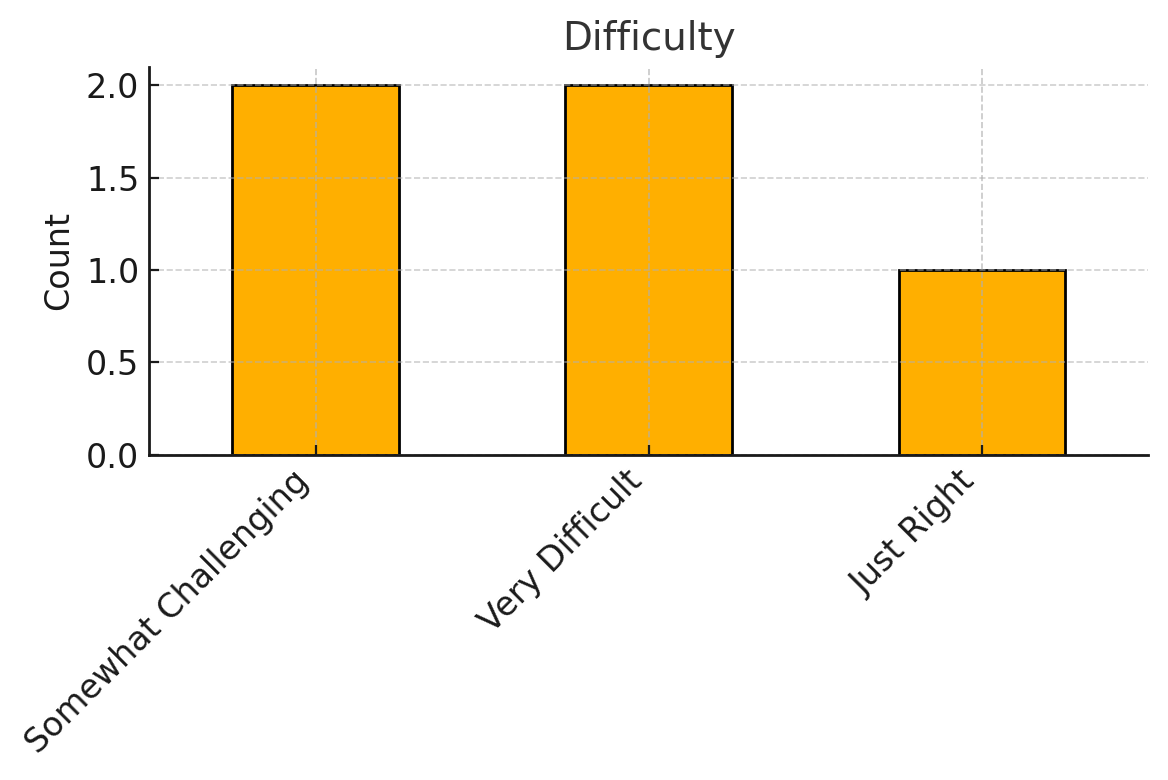
\includegraphics[width=0.3\textwidth]{./gp_test1.png}
    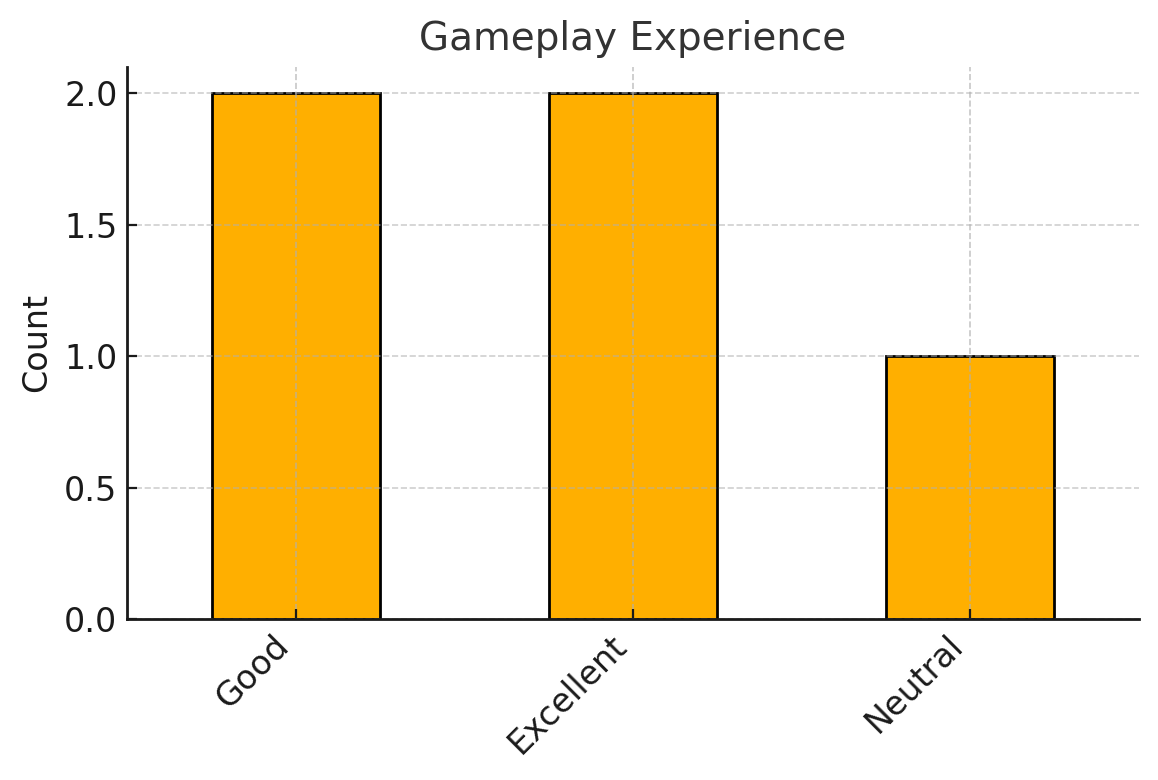
\includegraphics[width=0.3\textwidth]{./gp_test2.png}
    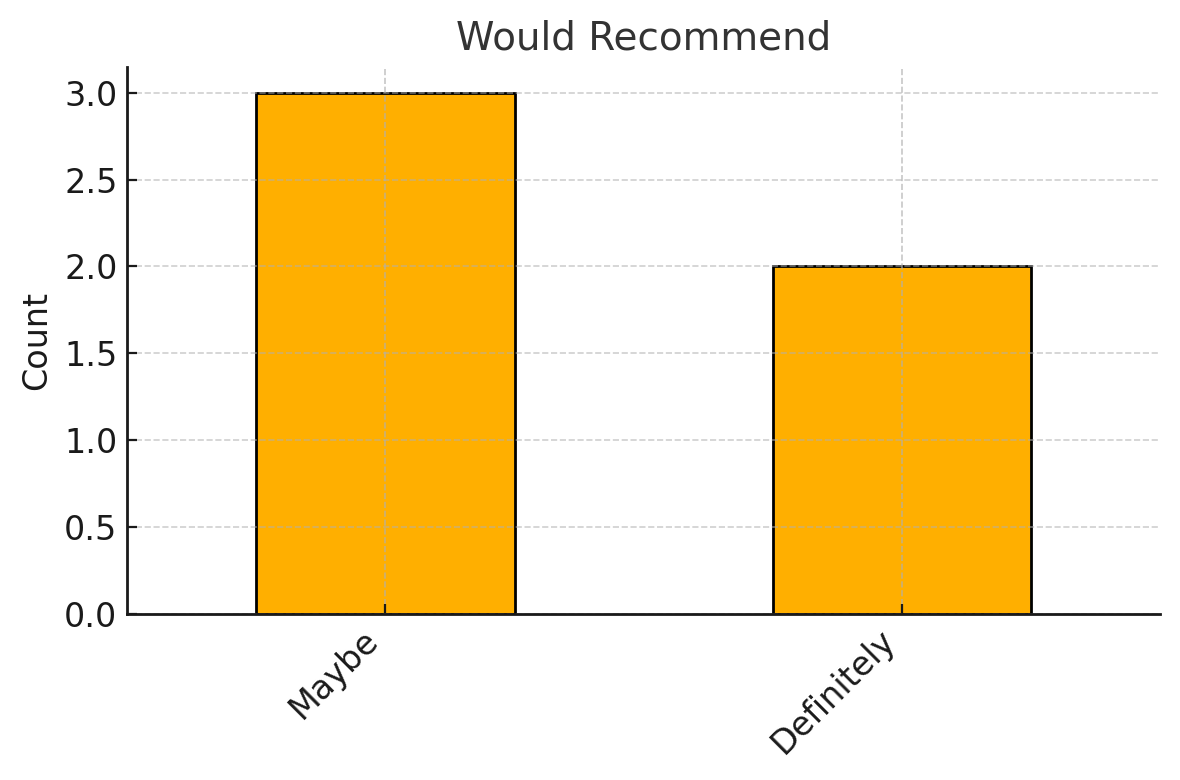
\includegraphics[width=0.3\textwidth]{./gp_test3.png}
    \caption{Results of the Gameplay Survey.}
    \label{fig:gp}
\end{figure}

\bibliographystyle{acm}
\bibliography{references}

\section{Appendix}

\paragraph{Testing}

\subparagraph{Voice of Customer}
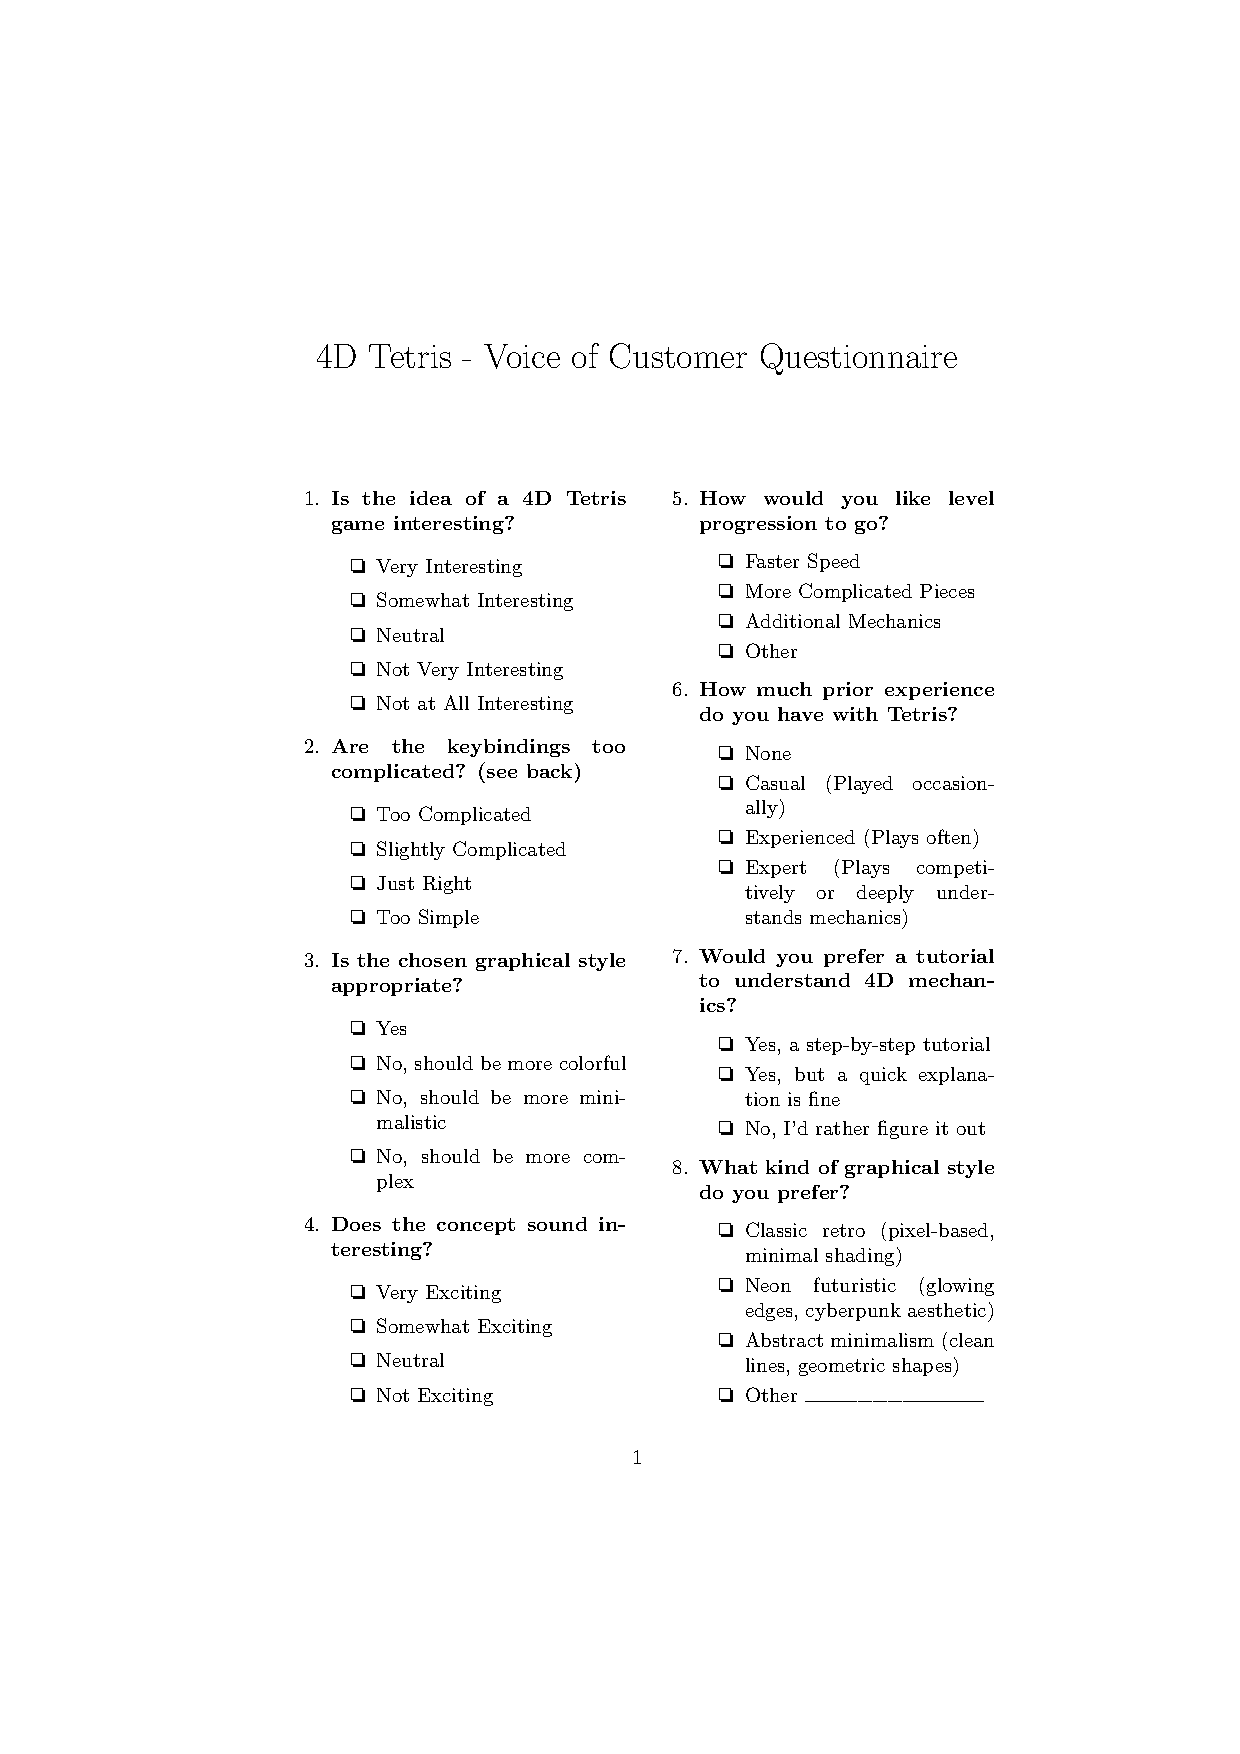
\includepdf{4d_tetris_questionnaire.pdf}

\begin{landscape}
    \subparagraph{Results}
    \begingroup\tiny 
        \begin{longtable}{lllllllll}
            \toprule
            \textbf{User} & \textbf{Idea Interest} & \textbf{Keybindings Complexity} & \textbf{Graphical Style Appropriate} & \textbf{Concept Interest} & \textbf{Level Progression} & \textbf{Tetris Experience} & \textbf{Tutorial Preference} & \textbf{Preferred Graphical Style} \\
            \midrule
            \endfirsthead
            \toprule
            \textbf{User} & \textbf{Idea Interest} & \textbf{Keybindings Complexity} & \textbf{Graphical Style Appropriate} & \textbf{Concept Interest} & \textbf{Level Progression} & \textbf{Tetris Experience} & \textbf{Tutorial Preference} & \textbf{Preferred Graphical Style} \\
            \midrule
            \endhead
            User 1 & Very Interesting & Too Simple & Yes & Neutral & More Complicated Pieces & Casual & Step-by-Step Tutorial & Neon Futuristic \\
            User 2 & Not Very Interesting & Just Right & No, should be more colorful & Very Exciting & Faster Speed & Casual & Quick Explanation & Abstract Minimalism \\
            User 3 & Neutral & Just Right & Yes & Very Exciting & Faster Speed & Expert & Quick Explanation & Abstract Minimalism \\
            User 4 & Somewhat Interesting & Just Right & No, should be more colorful & Somewhat Exciting & Additional Mechanics & Casual & Quick Explanation & Classic Retro \\
            User 5 & Very Interesting & Just Right & No, should be more complex & Not Exciting & More Complicated Pieces & Casual & Quick Explanation & Classic Retro \\
            User 6 & Very Interesting & Just Right & Yes & Very Exciting & Faster Speed & Experienced & No Tutorial Needed & Neon Futuristic \\
            User 7 & Very Interesting & Too Complicated & Yes & Somewhat Exciting & Faster Speed & Expert & Quick Explanation & Classic Retro \\
            User 8 & Neutral & Too Complicated & No, should be more minimalistic & Somewhat Exciting & Additional Mechanics & Experienced & Step-by-Step Tutorial & Neon Futuristic \\
            User 9 & Somewhat Interesting & Too Complicated & Yes & Very Exciting & Faster Speed & Experienced & Quick Explanation & Other \\
            User 10 & Neutral & Slightly Complicated & Yes & Somewhat Exciting & Faster Speed & None & Step-by-Step Tutorial & Neon Futuristic \\
            User 11 & Very Interesting & Slightly Complicated & Yes & Very Exciting & More Complicated Pieces & Experienced & Step-by-Step Tutorial & Neon Futuristic \\
            User 12 & Not Very Interesting & Slightly Complicated & Yes & Somewhat Exciting & Additional Mechanics & Expert & Step-by-Step Tutorial & Neon Futuristic \\
            User 13 & Neutral & Just Right & No, should be more complex & Somewhat Exciting & Additional Mechanics & Casual & Step-by-Step Tutorial & Neon Futuristic \\
            User 14 & Very Interesting & Slightly Complicated & No, should be more minimalistic & Somewhat Exciting & Faster Speed & Experienced & No Tutorial Needed & Neon Futuristic \\
            User 15 & Very Interesting & Slightly Complicated & No, should be more colorful & Very Exciting & Additional Mechanics & Expert & Quick Explanation & Other \\
            User 16 & Very Interesting & Just Right & No, should be more minimalistic & Neutral & Faster Speed & Experienced & Quick Explanation & Neon Futuristic \\
            User 17 & Very Interesting & Too Complicated & No, should be more minimalistic & Very Exciting & Faster Speed & Experienced & Step-by-Step Tutorial & Other \\
            User 18 & Somewhat Interesting & Just Right & Yes & Very Exciting & Additional Mechanics & Experienced & Step-by-Step Tutorial & Other \\
            User 19 & Somewhat Interesting & Too Complicated & No, should be more minimalistic & Very Exciting & More Complicated Pieces & Casual & Step-by-Step Tutorial & Classic Retro \\
            User 20 & Very Interesting & Too Simple & No, should be more colorful & Somewhat Exciting & Additional Mechanics & Casual & Step-by-Step Tutorial & Classic Retro \\
            User 21 & Somewhat Interesting & Just Right & No, should be more minimalistic & Somewhat Exciting & Additional Mechanics & Experienced & Quick Explanation & Classic Retro \\
            User 22 & Very Interesting & Too Complicated & No, should be more minimalistic & Very Exciting & More Complicated Pieces & Experienced & Quick Explanation & Classic Retro \\
            User 23 & Very Interesting & Too Complicated & Yes & Somewhat Exciting & Faster Speed & Expert & Quick Explanation & Classic Retro \\
            User 24 & Very Interesting & Just Right & Yes & Very Exciting & More Complicated Pieces & Expert & Step-by-Step Tutorial & Abstract Minimalism \\
            User 25 & Somewhat Interesting & Just Right & Yes & Somewhat Exciting & Faster Speed & Experienced & No Tutorial Needed & Classic Retro \\
            User 26 & Neutral & Just Right & Yes & Very Exciting & Faster Speed & Experienced & Quick Explanation & Neon Futuristic \\
            User 27 & Very Interesting & Just Right & No, should be more minimalistic & Somewhat Exciting & Other & Experienced & Quick Explanation & Abstract Minimalism \\
            User 28 & Somewhat Interesting & Too Complicated & No, should be more minimalistic & Very Exciting & More Complicated Pieces & Experienced & Quick Explanation & Classic Retro \\
            User 29 & Somewhat Interesting & Slightly Complicated & Yes & Neutral & Additional Mechanics & Experienced & Step-by-Step Tutorial & Abstract Minimalism \\
            User 30 & Very Interesting & Too Complicated & No, should be more colorful & Very Exciting & More Complicated Pieces & Experienced & Step-by-Step Tutorial & Classic Retro \\
            User 31 & Somewhat Interesting & Just Right & Yes & Very Exciting & Additional Mechanics & Expert & Step-by-Step Tutorial & Classic Retro \\
            User 32 & Very Interesting & Just Right & Yes & Very Exciting & More Complicated Pieces & Casual & Quick Explanation & Abstract Minimalism \\
            User 33 & Very Interesting & Slightly Complicated & Yes & Neutral & More Complicated Pieces & Casual & Step-by-Step Tutorial & Neon Futuristic \\
            User 34 & Not Very Interesting & Too Complicated & Yes & Neutral & More Complicated Pieces & None & Step-by-Step Tutorial & Abstract Minimalism \\
            User 35 & Not Very Interesting & Slightly Complicated & No, should be more complex & Very Exciting & Faster Speed & Experienced & Step-by-Step Tutorial & Abstract Minimalism \\
            User 36 & Neutral & Slightly Complicated & Yes & Somewhat Exciting & Additional Mechanics & None & Step-by-Step Tutorial & Abstract Minimalism \\
            User 37 & Very Interesting & Just Right & No, should be more colorful & Neutral & Faster Speed & Casual & No Tutorial Needed & Classic Retro \\
            User 38 & Very Interesting & Just Right & No, should be more minimalistic & Somewhat Exciting & Faster Speed & Experienced & Quick Explanation & Classic Retro \\
            User 39 & Somewhat Interesting & Just Right & Yes & Somewhat Exciting & More Complicated Pieces & Casual & Step-by-Step Tutorial & Abstract Minimalism \\
            User 40 & Somewhat Interesting & Slightly Complicated & No, should be more complex & Very Exciting & Faster Speed & Experienced & Step-by-Step Tutorial & Abstract Minimalism \\
            User 41 & Very Interesting & Too Complicated & No, should be more complex & Very Exciting & Other & None & Step-by-Step Tutorial & Other \\
            User 42 & Somewhat Interesting & Just Right & Yes & Neutral & Other & None & Step-by-Step Tutorial & Neon Futuristic \\
            User 43 & Very Interesting & Just Right & Yes & Neutral & Other & Experienced & Step-by-Step Tutorial & Neon Futuristic \\
            User 44 & Not Very Interesting & Just Right & Yes & Somewhat Exciting & More Complicated Pieces & Casual & Step-by-Step Tutorial & Abstract Minimalism \\
            User 45 & Very Interesting & Just Right & Yes & Very Exciting & Faster Speed & Casual & Step-by-Step Tutorial & Neon Futuristic \\
            User 46 & Somewhat Interesting & Slightly Complicated & Yes & Very Exciting & Other & Experienced & Quick Explanation & Other \\
            User 47 & Very Interesting & Just Right & No, should be more colorful & Somewhat Exciting & More Complicated Pieces & Experienced & Quick Explanation & Abstract Minimalism \\
            User 48 & Somewhat Interesting & Slightly Complicated & No, should be more colorful & Neutral & Other & Casual & Step-by-Step Tutorial & Neon Futuristic \\
            User 49 & Somewhat Interesting & Too Complicated & Yes & Neutral & Other & Experienced & Step-by-Step Tutorial & Abstract Minimalism \\
            User 50 & Very Interesting & Too Complicated & Yes & Somewhat Exciting & Additional Mechanics & None & Quick Explanation & Abstract Minimalism \\
            \bottomrule
            
        \end{longtable}
    \endgroup   
 \end{landscape}

\subparagraph{Gameplay Testing}
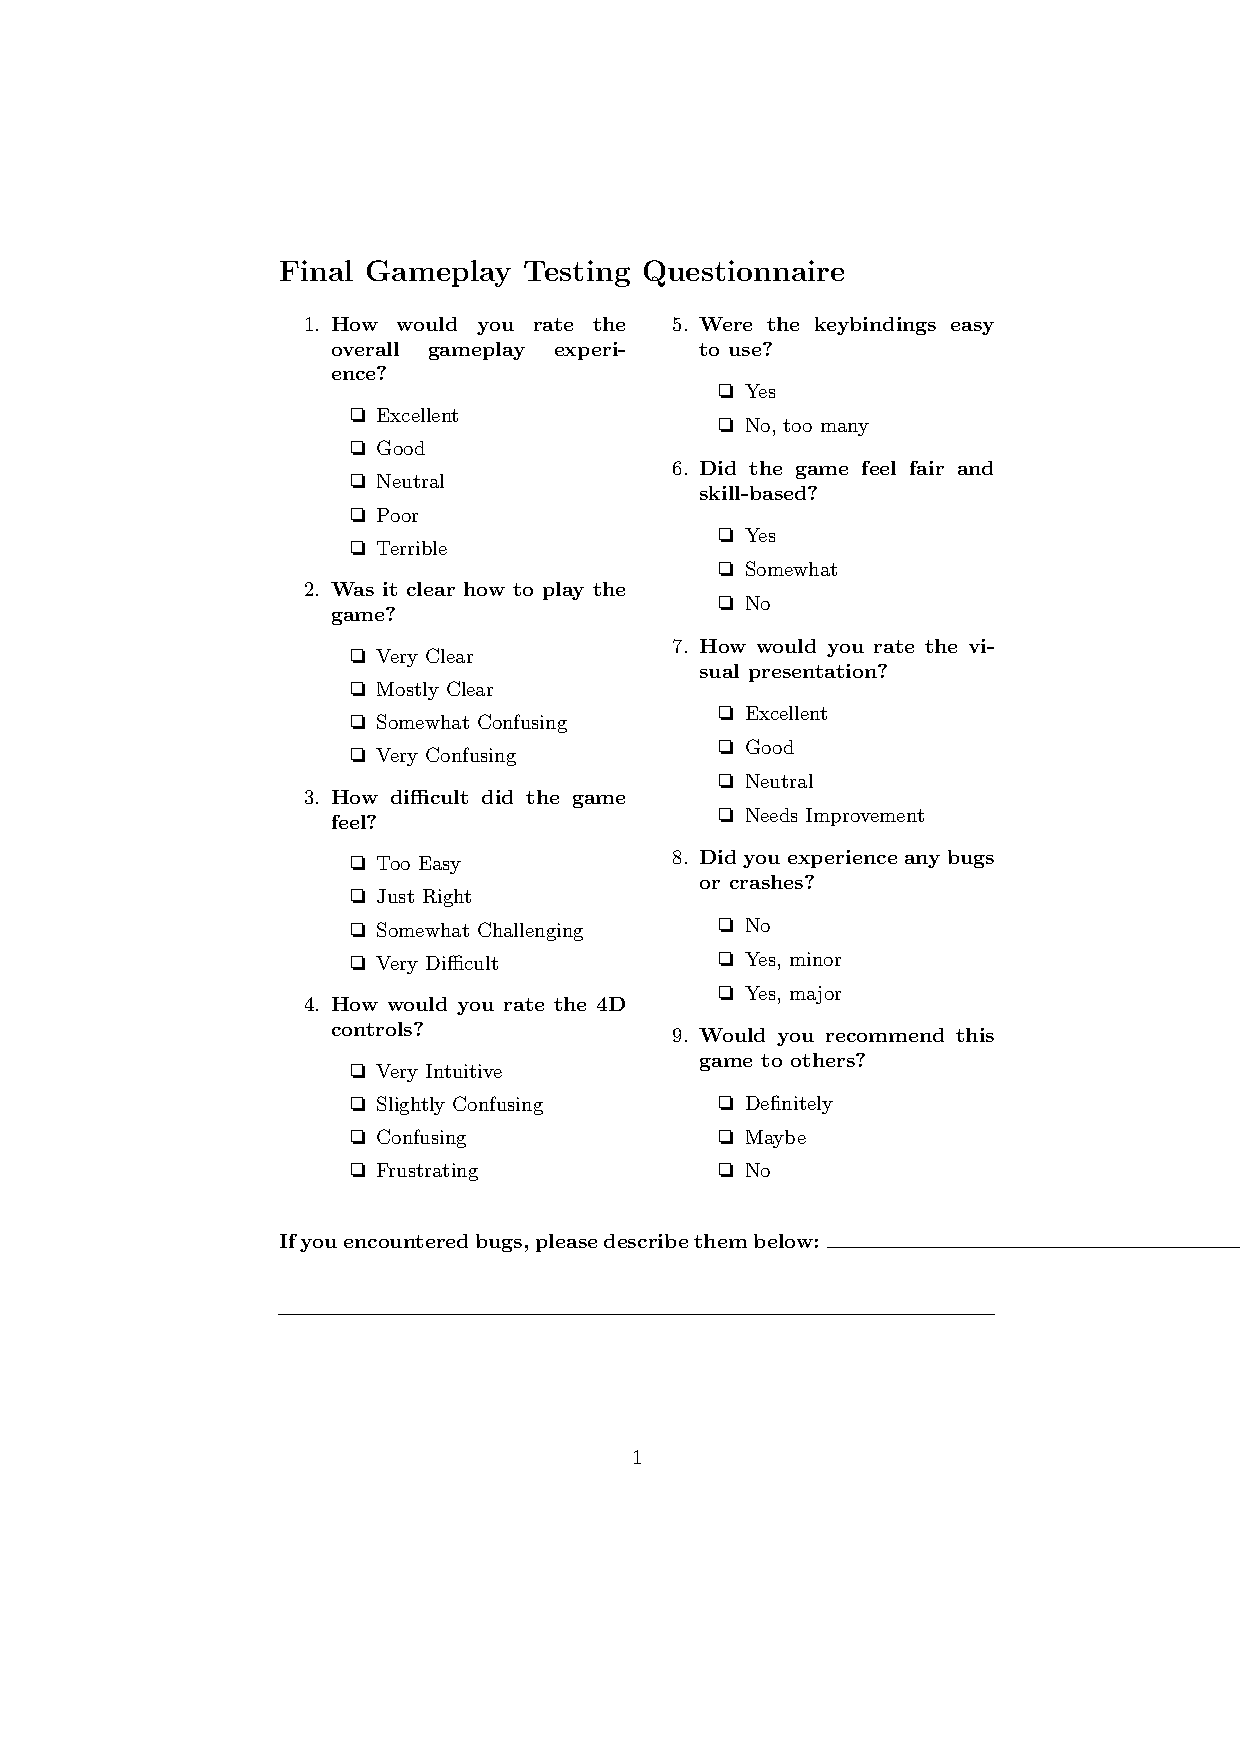
\includepdf{final_test.pdf}

\begin{landscape}
\subparagraph{Results}
\begingroup\tiny 
    \begin{longtable}{lllllllllll}
    \toprule
    \textbf{User} & \textbf{Gameplay Experience} & \textbf{Clarity of Instructions} & \textbf{Difficulty} & \textbf{4D Controls} & \textbf{Keybindings} & \textbf{Fairness} & \textbf{Visuals} & \textbf{Bugs Encountered} & \textbf{Would Recommend} & \textbf{Bug Description} \\
    \midrule
    \endfirsthead
    \toprule
    \textbf{User} & \textbf{Gameplay Experience} & \textbf{Clarity of Instructions} & \textbf{Difficulty} & \textbf{4D Controls} & \textbf{Keybindings} & \textbf{Fairness} & \textbf{Visuals} & \textbf{Bugs Encountered} & \textbf{Would Recommend} & \textbf{Bug Description} \\
    \midrule
    \endhead
    User 1 & Good & Very Clear & Somewhat Challenging & Slightly Confusing & Yes & Somewhat & Excellent & Yes, minor & Maybe & Minor glitch with the rectangle on the sides \\
    User 2 & Good & Somewhat Confusing & Very Difficult & Slightly Confusing & Yes & Yes & Good & Yes, major & Maybe & Crash on restart \\
    User 3 & Neutral & Somewhat Confusing & Very Difficult & Slightly Confusing & Yes & Yes & Neutral & No & Definitely &  \\
    User 4 & Excellent & Mostly Clear & Somewhat Challenging & Very Intuitive & No, too many & Yes & Good & Yes, minor & Maybe & Crash on restart \\
    User 5 & Excellent & Mostly Clear & Just Right & Very Intuitive & Yes & Somewhat & Good & Yes, major & Definitely & Crash on restart \\
    \bottomrule
    \end{longtable}
\endgroup
\end{landscape}
\end{document}